\documentclass[a4paper,12pt]{article}
%\usepackage[utf8x]{inputenc}
\usepackage{fontspec}
\usepackage{xeCJK}
\usepackage{xcolor,colortbl}
\setCJKmainfont{DFMing-Md-HK-BF.ttf}
%% Language and font encodings
%\usepackage[english]{babel}
%\usepackage[T1]{fontenc}
\usepackage{minted}
%\usepackage{indentfirst}
%% Sets page size and margins
\usepackage[a4paper,top=2.5cm,bottom=2.5cm,left=2.5cm,right=2.5cm,marginparwidth=0.5cm]{geometry}
\usepackage{hyperref}
\renewcommand{\figurename}{圖}
\renewcommand{\figureautorefname}{圖}
\renewcommand{\tablename}{表}
\renewcommand{\tableautorefname}{表}
\setlength{\parindent}{2em}
\setlength{\parskip}{0.5em}
\renewcommand{\baselinestretch}{1.4}
%\usepackage[explicit]{titlesec}
%\usepackage{tikz}
%\usetikzlibrary{shapes,shadows,calc}
%\usepackage{lipsum}

%\definecolor{visgreen}{rgb}{0.733, 0.776, 0}

% the tikz picture that will be used for the title formatting
% \SecTitle{<signal direction>}{<node anchor>}{<node horiz, shift>}{<node x position>}{#5}
% the fifth argument will be used by \titleformat to write the section title using #1
%\newcommand\SecTitle[5]{%
%\begin{tikzpicture}[overlay,every node/.style={signal, draw, text=white, signal to=nowhere}]
%  \node[visgreen,fill, signal to=#1, inner sep=0.5em,
%    text=white,font=\Large\sffamily,anchor=#2,
%    xshift=\the\dimexpr-\marginparwidth-\marginparsep-#3\relax] 
%    at (#4,0) {#5};
%\end{tikzpicture}%
%}
%\titleformat{name=\section,page=odd}
%{\normalfont}{}{0em}
%{\SecTitle{east}{west}{16pt}{0}{#1}}[\addvspace{4ex}]

%\titleformat{name=\section,page=even}
%{\normalfont\sffamily}{}{0em}
%{\SecTitle{west}{east}{14pt}{\paperwidth}{#1}}[\addvspace{4ex}]



%% Useful packages
%\usepackage{amsmath}
%\usepackage{graphicx}
%\usepackage[colorinlistoftodos]{todonotes}
\definecolor{bgc}{rgb}{0.95,0.95,0.95}
\definecolor{LightCyan}{rgb}{0.88,1,1}
%\usepackage[colorlinks=true, allcolors=blue]{hyperref}
%\usepackage{abstract}
\renewcommand{\abstractname}{}%}\large 摘要}
\newcommand{\cc}{C\texttt{++}}

\newminted{cpp}{xleftmargin=.8cm,linenos,baselinestretch=1.2,autogobble=true,tabsize=4,showtabs=false,frame=single,framesep=10pt}
\newminted[inside]{cpp}{tabsize=4,autogobble=true,baselinestretch=1.2}

\title{2017年程式設計先修暑期夏令營\\課程大綱(助教版)}
%\author{王佳盈 梁家萁 侯怡安 朱睿謙 巫鈺瑩 周身鴻}
\begin{document}
\maketitle
%\begin{abstract}
%\chapter{前言}
我喜歡寫程式,寫程式可以說是學習和電腦打交道的過程。在寫程式的過程中,會發現電腦可以說得上是一位忠實、公正,又極有耐心的朋友,這些特質電腦發揮得極其盡緻,世間的朋友很難比得上。首先它非常客觀公正,無論情況多麼撲朔迷離,它仍然會在其中依循既定的原則而行,絕沒有一絲一豪偏離軌道;也不管你的程式功力多麼高深,程式寫得多麼巨大華麗,對於那豪不起眼的一點小小錯誤,它也絕不會輕易地把你放過,這是它忠實、公正的特質。另外,不管你的程式能力多麼拙劣,永無止盡的在相同的小錯誤中周旋,它也絕不失去耐心,乃至發出一點點怒火,仍然保持著冷靜沈著,一再地把最忠實而相同的錯誤訊息反應給你,這樣的耐心幾乎無人能及。如果要說它的一些缺點,大概就是有點不盡人情,有時候迂腐得可以。

寫程式跟學習世間的技能,過程非常一致。一個人學習游泳,學習騎腳踏車,如果沒有真正下水或上路練習,而只是詳細閱讀教學手冊,要真正在水中得到游泳的樂趣,或者在路上騎乘的快感,那幾乎是不太可能的事。同樣地,一個學習寫程式的人,如果沒有真正上機練習,而光是閱讀程式教學的書籍,要真正具備寫作程式的能力,那也是非常困難的事情。初學游泳的人,總是要在水中嗆幾口水;初學騎腳踏車的人,也不免有不穩或摔倒的時候,這都是學習過程普遍發生的事情。相同地,初學程式的人,總會有弄不清頭緒,在不解的錯誤中周旋的時候,這是一種除錯和學習的過程,不用因此而灰心喪志,只要持續努力,慢慢會掌握寫程式的一些絕竅。

我因為喜歡寫程式,後來也有機會開始擔任C/\cc{}程式的教學。因為了解學習程式必須實際練習,所以也一直在尋找合適的學習資源。現在網路非常發達,資訊詳盡而多元,要找到一些學習資源並不太難,但是在尋找C/\cc{}的學習資源的過程中,發現大部份的學習工具和平台多是英語介面,對於國內很多學生來說,還是有一些不容易跨越的門檻。後來在尋覓的過程中,發現了銘傳大學謝育平老師所寫作的「瘋狂程設」,這個平台不僅完全使用中文,而且還可以把許多教學、作業和解題的過程融合在一個系統中,不僅對初學程式的人極有幫助,對於程式教學的老師來說,也提供非常有用的資源,可以達到事半功倍的效果。後來也承蒙謝老師的幫助,連續幾年開課,我都一直使用這個學習平台,作為教學的輔助資源。

「瘋狂程設」的平台中,提供了很多練習題目,可以讓學習程式的人練習,而老師也可以使用這個系統,不斷開發新的題目。對於剛入門的同學來說,「瘋狂程設」有一個程式練習廣場,裡面很有系統地提供一些基礎的題目,讓初學的人練習解題,漸次深入,這就好像玩遊戲過關斬將一樣,讓學習程式也可以變得很有樂趣。對於老手來說,這些題目可能不堪一擊,但對初學者來說,很多人經常卡關,面對題目不知所措,甚至充滿了挫折。這本書的內容,主要就是針對程式練習廣場的題目,提供詳盡的思惟過程和解題參考,可以作為初學者的破關攻略,也可以從中看到各種不同的解題技巧。

這本書能夠完成,還要特別感謝實驗室幾位研究生,包括梁家萁、侯怡安、朱睿謙、巫鈺瑩、以及周身鴻等人。我讓他們每個人先練習撰寫書中的一小部份章節,一方面他們可以練習,一方面我也可以減輕一些負擔,等他們寫完各章節之後,我再整體看過並做修改。所以這本書能夠完成,也要非常感謝這些同學的幫忙。

我希望這本書可以幫助到初學C/\cc{}程式的人,也希望提供給程式教學的老師作為教學的參考,減輕彼此教和學的負擔和困難,乃至達到事半功倍的效果。書中的內容,主要針對問題如何思考和解答來做說明,所以不是完整的教科書,很多C/\cc{}語言基本的概念,還是應該要參閱其他的書籍和資源。

另外,寫程式要有相對應的開發工具,在教學上,我習慣使用的整合開發環境是Code::Blocks,這是一套跨平台的自由軟體,功能實用而且豐富;而編譯程式用的編譯器則是使用mingw,這是gcc移植到Windows的版本,也可以說是非常普及而強大的編譯工具。讀者只要連到Code::Blocks的官網,可以直接下載內含mingw的Code::Blocks版本,非常便利。本書第一部份也會針對Code::Blocks的安裝以及瘋狂程設的使用做一些說明。

我必須再次強調,學習程式一定要自己思考和練習,如果只是光看而不練的話,實際遇到問題,還是做不出來的。因此同學在使用本書的時候,除了閱讀之外,也要花一些時間自己思考,並且實際上機練習解題,務求每一個步驟都充份了解和熟悉,這樣才能達到理想的功效。

對於本書的內容,如果有什麼修正建議或錯誤指正,還請不吝提供給我們作為修正的參考,連絡方式,可以寄信到\ \href{mailto:jywglady@gmail.com}{jywglady@gmail.com}\ 電子信箱,我們先在此感謝您的幫忙。最後敬祝大家學習愉快,一切平安吉祥。

\begin{flushright}
	王佳盈 寫於 2018/06
\end{flushright}

%\end{abstract}
\ \\ \\ \\ \\ \\
\begin{center}
	本課程穫教育部扎根高中職資訊科學教育計畫補助
\end{center} 
\newpage
這份講義,僅提供給老師和助教作為教學參考之用,
講義的內容,主要針對瘋狂程設上的學習問題,
提供參考的思考流程和程式解答,供作教學參考之用。

這份講義還在修改階段,如果有什麼修正的建議,可以提供給我們,感謝大家。

\newpage
\setcounter{tocdepth}{2}
\tableofcontents


\section{8/14(一)上午:環境設定}

%\subsection{上午:環境設定}
\subsection{行政事項}
\begin{enumerate}
	\item i-learning登入測試
		\subitem 網頁版
		\subitem 下載app版
		\begin{figure}[H]
			\centering
			
\includegraphics[width=3.5cm]{fig/QRcode}
		\end{figure}
	\item 藍芽點名
	\item 宣傳保溫課程、說明校園參訪&校外參訪

\end{enumerate}
\subsection{認識新朋友}
\begin{enumerate}
	\item 老師、助教自我介紹
	\item 同學自我介紹
\end{enumerate}
	

\subsection{實力測驗(前測)}
\begin{enumerate}

\item 動手玩程式
\subitem \href{https://studio.code.org/courses}{冰雪奇緣遊戲}(15分鐘)
\end{enumerate}

\subsection{環境設定}
\begin{enumerate}
\item Code::Blocks
\subitem 安裝說明
\item 瘋狂程設
\subitem 註冊
\subitem 加課
\subitem 桌機板	
\end{enumerate}

\section{8/14(一)下午:基本語法}

	\subsection{輸入、輸出(cin, cout)}
	\subsection{四則運算}
	
\begin{enumerate}
	\item 講解︰A001:Hello World
	\begin{enumerate}
	\item 題目說明:
	\subitem 請在命令視窗中印出 ``Hello World!"。
	
	\item 解題思維:
	\subitem 本題直接使用cout或printf函數印出想要顯示的文字即可。
	
	\item 程式碼:
	\begin{cppcode}
		#include <iostream>
		
		using namespace std;
		
		int main()
		{
			cout << "Hello World!";
			return 0;
		}
	\end{cppcode}
	\end{enumerate}
	
	\item 練習︰JT-01︰我可以把程式學好
		\begin{enumerate}
			\item 題目說明:
			\subitem 請印出字串 "Programming is easy!"
			
			\item 解題思維:
			\subitem 本題直接使用cout或printf函數印出想要顯示的文字即可。
			
			\item 程式碼:
			\begin{cppcode}
				#include <iostream>
				
				using namespace std;
				
				int main()
				{
					cout << "Programming is easy!";
					return 0;
				}
				
			\end{cppcode}
		\end{enumerate}
	\item 講解︰F001:兩數相加%(第01關:變數與計算)
		\begin{enumerate}
			\item 題目說明:
			\subitem 輸入兩整數,輸出兩數之和。
			
			\item 解題思維:
			%\subitem
			\begin{enumerate}
			\item 先宣告兩個變數。
			\begin{inside}
			int a, b; // 宣告變數
			\end{inside}
			\item 使用cin取得使用者輸入的兩個數字。
			\begin{inside}
			cin >> a >> b; // 取得輸入的值, 存入a和b
			\end{inside}
			\item 將剛剛取得的兩個數字相加,並用cout輸出。
			\begin{inside}
			cout << a+b;
			\end{inside}
			\end{enumerate} 
			
			\item 程式碼:
			\begin{cppcode}
				#include <iostream>
				
				using namespace std;
				
				int main()
				{
					int a, b;
					cin >> a >> b;
					cout << a+b;
					return 0;	
				}
			\end{cppcode}
		\end{enumerate}
		
	\item 練習︰F019:長方形面積%(第01關:變數與計算)
		\begin{enumerate}
			\item 題目說明:
			\subitem 輸入長和寬,輸出面積。
			
			\item 解題思維:
			\subitem 與上題解題思維大致相同,只是兩數相加變為兩數相乘。
			
			\item 程式碼:
			\begin{cppcode}
				#include <iostream>
				
				using namespace std;
				
				int main()
				{
					int a, b;
					cin >> a >> b;
					cout << a*b;
					return 0;	
				}
			\end{cppcode}
		\end{enumerate}
		
	\item 練習︰G001:長寬高算體積
		\begin{enumerate}
			\item 題目說明:
			\subitem 輸入長方體的長寬高,輸出其體積。
			
			\item 解題思維:
			\subitem 與上題解題思維大致相同,變數改成三個,輸出將三數相乘。
			
			\item 程式碼:
			\begin{cppcode}
				#include <iostream>
				
				using namespace std;
				
				int main()
				{
					int a, b, c;
					cin >> a >> b >> c;
					cout << a*b*c;
					return 0;	
				}
			\end{cppcode}
		\end{enumerate}
		
	\item 講解︰M90H011:整數商餘%(第01關:變數與計算){\color{blue} (cout and printf) }
		\begin{enumerate}
			\item 題目說明:
			\subitem 
			輸入兩整數m和n,輸出m除以n之商及餘數。
			\item 解題思維:
			\begin{enumerate}
			\item  先宣告兩個變數m和n,再使用scanf取得使用者輸入的兩個整數。
			\begin{inside}
			int m, n;
			scanf("%d%d", &m, &n); 
			\end{inside}
			\item  將剛剛取得的整數m除以整數n,並用printf輸出所除結果之商及餘數。
			\begin{inside}
			printf("\n%d / %d = %d", m, n, m / n);
			printf("\n%d mod %d = %d", m, n, m % n);
			\end{inside}
			\end{enumerate}
			
			\item 程式碼:
			\begin{cppcode}
				#include <stdio.h>
				
				int main()
				{
					int m, n;
					scanf("%d%d", &m, &n); 
					printf("\n%d / %d = %d", m, n, m / n);
					printf("\n%d mod %d = %d", m, n, m % n);
					return 0;
				}
			\end{cppcode}
		\end{enumerate}
	
	\item 練習︰使用printf完成下列兩題
	\begin{enumerate}
		\item F001︰兩數相加
		\item F019 ︰長方形面積
	\end{enumerate}
\end{enumerate}



\section{8/15(二)上午:流程控制-分支}

	

\subsection{分支}

\subsubsection{if}
\begin{enumerate}
	\item 講解︰JA-001:兩數排序
		\begin{enumerate}
			\item 題目說明:
			\subitem 輸入a和b兩個數,將其依小到大的順序印出來。
			
			\item 解題思維:
			\begin{enumerate}
				\item 用if進行判斷,如果a大於b,則兩數交換。
				
				\item 交換兩數a和b,在\cc{}中可以直接使用swap函數,如果是在C裡面,則常用的方法是宣告另一個暫存變數t,然後使用以下敘述:
				\begin{inside}
				t=a; x=b; b=t;
				\end{inside}
			\end{enumerate}
			\item 程式碼:
			\begin{cppcode}
				#include <iostream>
				
				using namespace std;
				
				int main()
				{
					int a, b;
					cin >> a >> b;
					if (a>b) swap(a, b);
					cout << a << " " << b;
					return 0;
				}
					
			\end{cppcode}
		\end{enumerate}
	\item 講解︰A016:三數排序
		\begin{enumerate}
			\item 題目說明:
			\subitem 輸入三個正整數 a、b、c,將 a、b、c 從小排到大並輸出。
			
			\item 解題思維:
			\begin{enumerate}
			\item 先宣告三整數 a, b, c並輸入其值。
			\begin{inside}
			int a, b, c;
			cin >> a >> b >> c;
			\end{inside}
			\item 三數排序時,先比a和b,如果a>b則交換兩個數,使a<b,之後再比b和c,使b<c,此時c為最大值。最後再比較和調整一次a和b即可。
			\begin{inside}
			if (a>b) swap(a, b);
			if (b>c) swap(b, c);
			if (a>b) swap(a, b);
			\end{inside}
			\item 交換兩數x和y,在\cc{}中可以直接使用swap函數,如果是在C裡面,則常用的方法是宣告另一個暫存變數t,然後使用以下敘述:
			\begin{inside}
			t=x; x=y; y=t;
			\end{inside}
			\end{enumerate} 
			
			\item 程式碼:
			\begin{cppcode}
				#include <iostream>
				using namespace std;
				
				int main()
				{
					int a, b, c;
					cin >> a >> b >> c;
					if (a>b) swap(a, b);
					if (b>c) swap(b, c);
					if (a>b) swap(a, b);
					cout << a << " " << b << " " << c;
					return 0;
				}
			\end{cppcode}
		\end{enumerate}
	\item 練習︰JA-002:四數排序
		\begin{enumerate}
			\item 題目說明:
			\subitem 輸入a,b,c,d四個數,將其依小到大的順序印出來。
			
			\item 解題思維:
			\begin{enumerate}
				\item 將最大的整數置換到變數d。
				\item 對a,b,c由小到大進行三數排序。
			\end{enumerate}
			
			\item 程式碼:
			\begin{cppcode}
				#include <iostream>
				
				using namespace std;
				
				int main()
				{
					int a, b, c, d;
					cin >> a >> b >> c >> d;
					if (a>b) swap(a, b);
					if (b>c) swap(b, c);
					if (c>d) swap(c, d);
					if (a>b) swap(a, b);
					if (b>c) swap(b, c);
					if (a>b) swap(a, b);
					cout << a << " " << b << " " << c << " " << d;
					return 0;
				}
				
			\end{cppcode}
		\end{enumerate}
	
\end{enumerate}
		
\subsubsection{if else}
\begin{enumerate}
	\item 講解︰A025:判斷閏年%第04關:分支)
		\begin{enumerate}
			\item 題目說明:
			\subitem 輸入西元年,如果該年是閏年,則輸出Yes,若該年不是閏年,則輸出No。 (閏年的定義為,四年一閏,逢百不閏,逢四百又閏。例如西元1004年為閏年,西元1100年不是閏年,西元1600年是閏年)
			
			\item 解題思維:
			\subitem 宣告年份 year,接著再按照閏年的規則判斷是否為閏年就好。
			
			\item 程式碼:
			\begin{cppcode}
				#include <iostream>
				using namespace std;
				
				int main()
				{
					int year;
					cin >> year;
					if (year%400==0) cout << "Yes";
					else if (year%100==0) cout << "No";
					else if (year%4==0) cout << "Yes";
					else cout << "No";
					return 0;
				}
			\end{cppcode}
		\end{enumerate}
		
	\item 講解︰F021:奇偶數%(第04關:分支)
		\begin{enumerate}
			\item 題目說明:
			\subitem 輸入一整數,輸出其奇偶性。
			
			\item 解題思維:
			\subitem 判斷整數n是否為奇數的方法,可求其除以2的餘數,若非0即為奇數。
			\begin{inside}
			if (n%2) { /* n 為奇數 */ }
			\end{inside}
			
			\item 程式碼:
			\begin{cppcode}
				#include <iostream>
				using namespace std;
				int main()
				{
					int n;
					cin >> n;
					if (n%2) cout << "odd";
					else cout << "even";
					return 0;
				}
			\end{cppcode}
		\end{enumerate}
	
	\item 練習︰A006:輸入之正負零%(第04關:分支)
		\begin{enumerate}
			\item 題目說明:
			\subitem 輸入一整數 N,如果 N 大於 0,則輸出 N>0,如果 N 等於 0,則輸出 N=0,如果 N 小於 0,則輸出 N<0。
			
			\item 解題思維:
			\subitem 先宣告整數 N,輸入值之後再判斷是大於零、等於零還是小於零,分別印出相對的敘述。
			
			\item 程式碼:
			\begin{cppcode}
				#include <iostream>
				using namespace std;
				
				int main()
				{
					int n;
					cin >> n;
					if (n>0) cout << "N>0";
					else if (n==0) cout << "N=0";
					else cout << "N<0";
					return 0;
				}
			\end{cppcode}
		\end{enumerate}
	
\end{enumerate}
\subsubsection{switch {\color{blue} (若有多餘時間)}}

\section{8/15(二)下午:實驗室參訪}




\section{8/16(三)上午:流程控制-迴圈}

\subsection{迴圈}
\subsubsection {while}
\begin{enumerate}
	\item 講解︰JA-003:1+2+3+...+100
		\begin{enumerate}
			\item 題目說明:
			\subitem 使用 while 迴圈計算 1+2+3+...+100
			
			\item 解題思維:
			\begin{enumerate}
				\item 宣告一個初始值為零的變數sum=0,準備進行累加。
				\item 使用while迴圈,當符合while的執行條件(n<100)時,會重複執行累加計算,累加完之後會更新n的值,當n不滿足執行條件時,結束迴圈。
				
			\end{enumerate}
				\begin{cppcode}
				#include <iostream>
				
				using namespace std;
				
				int main()
				{
					int n=1, sum=0;
					while (n<=100) {
						sum += n; // 累加
						n++; // 更新n
					}
					cout << sum;
					return 0;
				}
				
			\end{cppcode}
		\end{enumerate}
		
	\item 練習:JA-004︰1+3+5+...+99
		\begin{enumerate}
			\item 題目說明:
			\subitem 使用 while 迴圈計算 1+3+5+...+99
			
			\item 解題思維:
			\subitem 使用while迴圈進行累加,只要(n<100)就對sum進行累加,每次累加完後,n加上2。
			
			\item 程式碼:
			\begin{cppcode}
				#include <iostream>
				
				using namespace std;
				
				int main()
				{
					int n=1, sum=0;
					while (n<100) {
						sum += n;
						n += 2;
					}
					cout << sum;
					return 0;
				}
				
			\end{cppcode}
		\end{enumerate}
	
\end{enumerate}

\subsubsection {for}
\begin{enumerate}
	\item 講解︰JA-005:1+2+3+...+100
		\begin{enumerate}
			\item 題目說明:
			\subitem 使用 for 迴圈計算 1+2+3+...+100
			
			\item 解題思維:
			\subitem for迴圈的用法是for(起始值; 條件式; 更新值),本題的for迴圈寫法如下:
			\begin{inside}
				for (int i=1; i<=100; i++) sum += i;
			\end{inside}
			意思是:i的起始值是1,當i<=100這個條件成立時的時候,會重複執行累加(sum += i;),並在累加完後更新i的值(i++)。此迴圈總共回會複執行100次累加的計算。
			
			\item 程式碼:
			\begin{cppcode}
				#include <iostream>
				
				using namespace std;
				
				int main()
				{
					int sum=0;
					for (int i=1; i<=100; i++) sum += i;
					cout << sum;
					return 0;
				}
				
			\end{cppcode}
		\end{enumerate}
	
	\item 練習︰JA-006:1+3+5+...+99
		\begin{enumerate}
			\item 題目說明:
			\subitem 使用 for 迴圈計算 1+3+5+...+99
			
			\item 解題思維:
			\subitem 使用for迴圈進行累加,只要(n<100)就對sum進行累加,n每次更新都加2。
			
			\item 程式碼:
			\begin{cppcode}
			#include <iostream>
			
			using namespace std;
			
			int main()
			{
				int sum=0;
				for (int i=1; i<100; i+=2) sum += i;
				cout << sum;
				return 0;
			}
				
			\end{cppcode}
		\end{enumerate}
	
\end{enumerate}

\subsubsection {應用題}
\begin{enumerate}
	\item 講解︰JT-04:印三角形函數
		\begin{enumerate}
			\item 題目說明:
			\subitem 輸入N,印出N列的星號(*),其中第I列有I個星,如執行範例所示。
			\subitem 範例輸入:5
			\subitem 範例輸出:
				\begin{figure}[H]
					\centering
					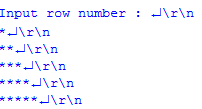
\includegraphics{fig/JT04fig}
				\end{figure}
			
			\item 解題思維:
			\subitem 
				這題需要使用雙重for迴圈。第一個迴圈計算現在要印第幾列,第二個迴圈計算要印幾個星。
			\item 程式碼:
			\begin{cppcode}
				#include <stdio.h>
				
				int main()
				{
					int n, i, j;
					printf("Input row number : \n");
					scanf("%d", &n);
					for (i=1; i<=n; i++) { // 迴圈1:第i列
						for(j=0; j<i; j++) { // 迴圈2:印i個星
							printf("*");
						}
						printf("\n");
					}
					return 0;
				}
					
			\end{cppcode}
		\end{enumerate}

	\item 練習︰JP-010-2:印倒三角形(無空白)
		\begin{enumerate}
			\item 題目說明:
			\subitem 輸入正整數n<=20,輸出一個n層的倒三角形。
			\subitem 範例輸入:5
			\subitem 範例輸出:
			\begin{figure}[H]
				\centering
				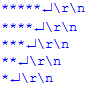
\includegraphics{fig/JP010fig}
			\end{figure}
			\item 解題思維:
			\subitem 印倒三角形時,第一列有n個星,下一列有n-1個星,以此列推,每換一列就少一個星,所以這題是要使用for迴圈來倒數。
			\item 程式碼:
			\begin{cppcode}
			#include <cstdio>
			
			int main()
			{
				int n, i, j;
				scanf("%d", &n);
				for (i=n; i>0; i--) { // 迴圈1:計算此列有i個星
					for(j=i; j>0; j--) { // 迴圈2:印出i個星
						printf("*");
					}
					printf("\n");
				}
				return 0;
			}
				
			\end{cppcode}
		\end{enumerate}
	
	\item 挑戰︰JT-40印等腰三角形
		\begin{enumerate}
			\item 題目說明:
			\subitem 輸入N,印出一個N列的等腰三角形,其中第I列有2*I-1個\#,如程式範例結果所示。
			\subitem 範例輸入:5
			\subitem 範例輸出:
			\begin{figure}[H]
				\centering
				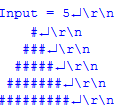
\includegraphics{fig/JT40fig}
			\end{figure}
			
			\item 解題思維:
			\begin{enumerate}
				\item 因為要印出N列,所以先寫一個執行N次的for迴圈,用變數row來計算現在是第幾列。
				\item 第row列要印出(n-row)個``空白",及(2*row-1)個``\#",所以分別用兩個for迴圈印``空白"及``\#"。
			\end{enumerate}
			
			\item 程式碼:
			\begin{cppcode}
				#include <stdio.h>
				
				int main()
				{
					int i, row, n;
					scanf("%d", &n);
					printf("Input = %d\n", n);
					for (row=1; row<=n; row++) {
						for (i=0; i<n-row; i++) printf(" ");
						for (i=0; i<2*row-1; i++) printf("#");
						printf("\n");
					}
					return 0;
				}
				
			\end{cppcode}
		\end{enumerate}

\end{enumerate}

\subsubsection {do while {\color{blue}(若有多餘時間)}}

\section{8/16(三)下午:函數}
\subsection{printf()格式輸出}
\begin{enumerate}
	\item 講解︰JB-02:九九乘法表
		\begin{enumerate}
			\item 題目說明:
			\subitem 印出如輸出之九九乘法表。
			\begin{figure}[h]
				\centering
				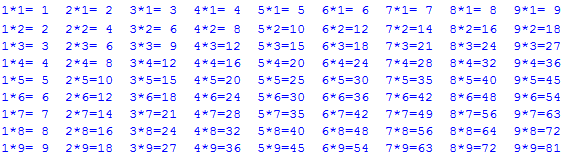
\includegraphics[width=12cm]{fig/JB02fig}
			\end{figure}
			\item 解題思維:
			\begin{enumerate}
				\item 先看第一列,會變動的數是``被乘數",而且變動是有規律的1,2,3...,9,所以我們寫一個會執行9次的for迴圈,讓變數j從1跑到9。變數j就是要輸出的``被乘數"。
				\begin{figure}[H]
					\centering
					
\includegraphics[width=12cm]{fig/JB02fig_2}
				\end{figure}
				\item 再來觀察``乘數",同一列的乘數是固定的,乘數隨著列改變,也就是說第i列的乘數是i。總共有9列,所以要寫一個會執行9次的for迴圈。變數i就是要輸出的``乘數"。
				\item ``乘積"只要將i, j 相乘就可以了。
				\item 這題使用printf()格式輸出比較容易。``\%2d"表示輸出時,會給這個整數兩給位數,當輸出的整數只有個位數的時候,十位數的位置會自動補上``空格"。
			\end{enumerate}
			
			\item 程式碼:
			\begin{cppcode}
			#include <cstdio>
			
			int main()
			{
				for (int i=1; i<=9; i++) {//第i列的乘數是i
					for(int j=1; j<=9; j++) {//每一列的被乘數j都從1~9
						printf("%d*%d=%2d  ", j, i, i*j);
					}
					printf("\n");
				}
				return 0;
			}
				
			\end{cppcode}
		\end{enumerate}
	
	\item 練習︰JA-007:九九乘法表 (兩排)
		\begin{enumerate}
			\item 題目說明:
			\subitem 印出九九乘法表,如輸出結果所示。
			\begin{figure}[h]
				\centering
				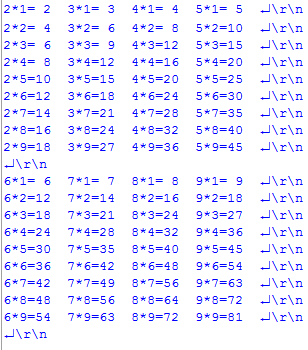
\includegraphics[height=6cm]{fig/JA007fig}
			\end{figure}
			\item 解題思維:
			\subitem 可以想成輸出兩個大群組的九九乘法表,當輸出第r (r=0, 1) 個群組時``被乘數"$=j+r\times4.$ (j=2, 3, 4, 5)。
			
			\item 程式碼:
			\begin{cppcode}
				#include <cstdio>
				
				int main()
				{
					for (int r=0; r<2; r++) {//兩個群組
						for (int i=1; i<=9; i++) {//第i列的乘數是i
							for(int j=2; j<=5; j++) {//被乘數=j+r*4
								printf("%d*%d=%2d  ", j+r*4, i, i*(j+r*4));
							}
							printf("\n");
						}
						printf("\n");
					}
					return 0;
				}
				
			\end{cppcode}
		\end{enumerate}
	
\end{enumerate}
\subsection{自訂函數}
\begin{enumerate}
	\item 講解︰JT-04印三角形函數
	\begin{enumerate}
		\item 題目說明:
		\subitem 輸入N,印出N列的星號(*),其中第I列有I個星,如執行範例所示。
		\subitem 範例輸入:5
		\subitem 範例輸出:
		\begin{figure}[H]
			\centering
			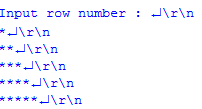
\includegraphics{fig/JT04fig}
		\end{figure}
		
		\item 解題思維:
		\begin{enumerate}
			\item 自己定義畫三角形的函數,使用這個函數時,需要輸入參數n,這樣函數才知道三角形有幾列。
			\item 將畫三角形的程式碼寫進函式裡,主程式main裡面只需要呼叫函數即可印出三角形。
		\end{enumerate}
		
		\item 程式碼:
		\begin{cppcode}
			#include <stdio.h>
			
			void triangle(int n);
			
			int main()
			{
				int n;
				printf("Input row number : \n");
				scanf("%d", &n);
				triangle(n);
				return 0;
			}
			
			void triangle(int n)
			{
				int i, j;
				for (i=1; i<=n; i++) {
					for (j=0; j<i; j++) { printf("*"); }
					printf("\n");
				}
			}
			
		\end{cppcode}
	\end{enumerate}
	
	\item 練習︰JP-010-2:印倒三角形(無空白)
	\begin{enumerate}
		\item 題目說明:
		\subitem 輸入正整數n<=20,輸出一個n層的倒三角形。
		\subitem 範例輸入:5
		\subitem 範例輸出:
		\begin{figure}[H]
			\centering
			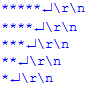
\includegraphics{fig/JP010fig}
		\end{figure}
		\item 解題思維:
		\begin{enumerate}
			\item 自己定義畫三角形的函數,使用這個函數時,需要輸入參數n,這樣函數才知道三角形有幾列。
			\item 將畫倒三角形的程式碼寫進函式裡,主程式main裡面只需要呼叫函數即可印出三角形。
		\end{enumerate}
		\item 程式碼:
		\begin{cppcode}
			#include <cstdio>
			
			void plot(int n);
			
			int main()
			{
				int n;
				scanf("%d", &n);
				plot(n);
				return 0;
			}
			
			void plot(int n)
			{
				int i, j;
				for (i=n; i>0; i--) {
					for(j=i; j>0; j--) {
						printf("*");
					}
					printf("\n");
				}
			}		
		\end{cppcode}
	\end{enumerate}
	
	\item 練習︰JT-40:印等腰三角形
		\begin{enumerate}
			\item 題目說明:
			\subitem 輸入N,印出一個N列的等腰三角形,其中第I列有2*I-1個\#,如程式範例結果所示。
			\subitem 範例輸入:5
			\subitem 範例輸出:
			\begin{figure}[H]
				\centering
				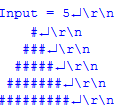
\includegraphics{fig/JT40fig}
			\end{figure}
			
			\item 解題思維:
			\begin{enumerate}
				\item 自己定義畫三角形的函數,使用這個函數時,需要輸入參數n,這樣函數才知道三角形有幾列。
				\item 將畫等腰三角形的程式碼寫進函式裡,主程式main裡面只需要呼叫函數即可印出三角形。
			\end{enumerate}
			
			\item 程式碼:
			\begin{cppcode}
				#include <stdio.h>
				
				void plot(int n);
				
				int main()
				{
					int n;
					scanf("%d", &n);
					printf("Input = %d\n", n);
					plot(n);
					
					return 0;
				}
				
				void plot(int n)
				{
					int i, row;
					for (row=1; row<=n; row++) {
						for (i=0; i<n-row; i++) printf(" ");
						for (i=0; i<2*row-1; i++) printf("#");
						printf("\n");
					}
				}
				
				
			\end{cppcode}
		\end{enumerate}
		
	
	
	\item 挑戰︰JT61:Game Over
		\begin{enumerate}
			\item 題目說明:
			\subitem 輸入整數 m 和 n,輸出以 \# 排成框,中間為 Game Over 之圖案,其中 m 為 G 之
			前和 r 之後與邊界的空格數,n 為文字與上下邊界的空格數。例如輸入 2 1,則輸出為
			\begin{figure}[h]
			\centering
			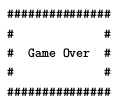
\includegraphics{fig/game_over_fig}
			\end{figure}
			\item 解題思維:
			\begin{enumerate}
				\item 第1列有11+2m個\#。
				\item 接下來n列頭尾是\#,中間有9+2m個空白。
				\item 再下一列是\#加m個空白,加Game Over,加m個空白和\#。
				\item 接下來n列頭尾是\#,中間有9+2m個空白。
				\item 最後一列有11+2m個\#。
			\end{enumerate}
			\item 程式碼:
		\begin{cppcode}
			#include <iostream>
			
			using namespace std;
			
			int main()
			{
				int m, n;
				cin >> m >> n;
				for (int i=0; i<11+2*m; i++) cout << "#"; // Row 1
				cout << endl;
				for (int r=0; r<n; r++) { // Next n rows
					cout << "#";
					for (int i=0; i<9+2*m; i++) cout << " ";
					cout << "#" << endl;
				}
				cout << "#"; // Middle row
				for (int i=0; i<m; i++) cout << " ";
				cout << "Game Over";
				for (int i=0; i<m; i++) cout << " ";
				cout << "#" << endl;
				for (int r=0; r<n; r++) { // Next n rows
					cout << "#";
					for (int i=0; i<9+2*m; i++) cout << " ";
					cout << "#" << endl;
				}
				for (int i=0; i<11+2*m; i++) cout << "#"; // Last row
				cout << endl;
				return 0;
			}
		
	\end{cppcode}
				
		\end{enumerate}
	
\end{enumerate}



\section{8/17(四)上午:遞迴}

\subsection{遞迴}
\begin{enumerate}
	\item 講解:JA-008:遞迴解1+2+...+n
		\begin{enumerate}
			\item 題目說明:
			\subitem 使用遞迴方式算出 1+2+...+n
			
			\item 解題思維:
			\subitem 假設$f(n)=1+2+...+n$,則遞迴的計算方法為$f(n)=n+f(n-1)$。
			
			\item 程式碼:
			\begin{cppcode}
				#include <cstdio>
				
				int f(int n);
				
				int main()
				{
					int n;
					scanf("%d", &n);
					printf("%d", f(n));
					return 0;
				}
				
				int f(int n)
				{
					if (n==1) return 1;
					return n + f(n-1);
				}
								
			\end{cppcode}
		\end{enumerate}
	
	\item 練習:A059:遞迴計算n階乘
		\begin{enumerate}
			\item 題目說明:
			\subitem 輸入一正整數N,輸出N!。其中$N! = 1\times2\times3\times...\times N$
			
			\item 解題思維:
			\subitem 假設函數$fact(n)=n! $,其遞迴的計算方式為$fact(n)=n\times fact(n-1)$。
			
			\item 程式碼:
			\begin{cppcode}
				#include<iostream>
				using namespace std;
				
				int fact(int n);

				int main()
				{
					int n;
					cin >> n;
					cout << fact(n);
					return 0;
				}

				int fact(int n)
				{
					if (n) return n * fact(n-1);
					else return 1;
				}

			\end{cppcode}
		\end{enumerate}
	
	\item 講解:A029︰費式數列
		\begin{enumerate}
			\item 題目說明:
			\subitem 費氏數列定義如下 $f(0)=0, f(1)=1, f(n)=f(n-1)+f(n-2)$。
			題目是從螢幕輸入一個正整數 n,輸出 $f(n)$。
			
			\item 解題思維:
			\begin{enumerate}
				\item 本題可用遞迴或非遞迴方式計算。
				\item 因為程式簡明易了,可直接觀看程式碼尋求理解。
			\end{enumerate}
			
			\item 程式碼:
			\begin{cppcode}
				#include <stdio.h>

				int f(int n);

				int main()
				{
					int n;
					scanf("%d", &n);
					printf("%d", f(n));
					return 0;
				}

				int f(int n)
				{
					if (n<2) return n;
					return f(n-1)+f(n-2);
				}
			\end{cppcode}
		\end{enumerate}
	
	\item 挑戰:JA-009:爬樓梯有幾種爬法
		\begin{enumerate}
			\item 題目說明:
			\subitem 小明爬樓梯,已知要爬的梯數有N階,但小明一次可以爬1~3階,請問總共有幾種爬法?
			
			\item 解題思維:
			\subitem
			當n=1, 2, 3時,分別有1, 2, 4種爬法,當n>3時,爬樓梯的方法為$f(n)=f(n-1)+f(n-2)+f(n-3)$。
			
			\item 程式碼:
			\begin{cppcode}
				#include <cstdio>
				
				int f(int n);
				
				int main()
				{
					int n;
					scanf("%d", &n);
					printf("%d", f(n));
					return 0;
				}
				
				int f(int n)
				{
					if (n==1) return 1;
					if (n==2) return 2;
					if (n==3) return 4;
					return f(n-1)+f(n-2)+f(n-3);
				}
			\end{cppcode}
		\end{enumerate}
	
	\item 講解:JB-04︰河內塔
	\begin{enumerate}
		\item 題目說明:
		\subitem 依課堂上講解之河內塔規則,從柱1移到柱3,柱2為輔助。輸入環的個數n,輸出所有移動過程。
		
		\item 解題思維:
		\subitem 河內塔的解法如下:
		\begin{enumerate}
			\item 當只有1個環的時候,直接把環搬到目標柱子上。
			\item 當有n個環的時候
			\begin{enumerate}
				\item 先將(n-1)層的河內塔搬到輔助的柱子上。
				\item 接著將第n個環搬到目標柱子上。
				\item 最後,再將(n-1)層的河內塔從輔助的柱子搬到目標柱子上。 
			\end{enumerate}
			
		\end{enumerate}
		
		\item 程式碼:
		\begin{cppcode}
			#include <iostream>
			
			using namespace std;
			
			void hanoi(int n, int from, int to, int buf);
			
			int main()
			{
				int n;
				cin >> n;
				hanoi(n, 1, 3, 2);
				return 0;
			}
			
			void hanoi(int n, int from, int to, int buf)
			{
				if (n==1) {
					cout << from << " => " << to << endl;
				} else {
				hanoi(n-1, from, buf, to);
				cout << from << " => " << to << endl;
				hanoi(n-1, buf, to, from);
			}
		}
	\end{cppcode}
\end{enumerate}

	
	
	
	
\end{enumerate}

\section{8/17(四)下午:陣列}

\subsection{陣列}
\begin{enumerate}
	\item 講解:A030︰百數反印
		\begin{enumerate}
			\item 題目說明:
			\subitem 輸入 100 個正整數,反向印出此 100 個數。
			
			\item 解題思維:
			\subitem 本題使用陣列儲存 100 個數,再反向印出即可,是很基本的題目。
			
			\item 程式碼:
			\begin{cppcode}
				#include<iostream>
				using namespace std;
				int main()
				{
					int data[100];
					for (int i=0; i<100; i++) cin >> data[i];
					for (int i=99; i>=0; i--) cout << " " << data[i];
					return 0;
				}
			\end{cppcode}
		\end{enumerate}
	
	\item 講解︰JT-30︰排序
		\begin{enumerate}
			\item 題目說明:
			\subitem 輸入N及N個數 (N<100),將N個數從小到大印出來。
			
			\item 解題思維:
			\subitem 本題是練習排序的演算法。基本上排序的演算法很多,以下程式使用\href{https://zh.wikipedia.org/wiki/%E5%86%92%E6%B3%A1%E6%8E%92%E5%BA%8F}{氣泡排序法},
			這也是最基本的排序演算法之一。在程式中,i 的範圍可以從 0
			到 n-2,或則倒過來從 n-1 到 1 也可以,基本上就是要執行 n-1 輪的意思,但是 i 的
			範圍寫法不同,j 的上限寫法也跟著(有)一些變化,這是在閱讀參考連結時,應注意的地
			方。
			
			\item 程式碼:
			\begin{cppcode}
				#include <stdio.h>
			
				int main()
				{
					int i, j, t, n, a[100];
					scanf("%d", &n);
					for (i=0; i<n; i++) scanf("%d", a+i);
					for (i=n-1; i>0; i--) {
						for (j=0; j<i; j++) {
							if (a[j]>a[j+1]) {
								t=a[j];
								a[j]=a[j+1];
								a[j+1]=t;
							}
						}
					}
					printf("%d", a[0]);
					for (i=1; i<n; i++) printf(" %d", a[i]);
					return 0;
				}
			\end{cppcode}
		\end{enumerate}
	
\end{enumerate}


\chapter{安裝與設定}

工欲善其事,必先利其器。在學習程式語言之前,也要先設定好程式的學習環境。這一章會教同學如何安裝及設定本書所使用的學習環境,首先說明如何安裝「Code::Blocks」以及「瘋狂程設」;其次,說明如何註冊瘋狂程設的帳號,並針對開課及修課的需要,說明如何在瘋狂程設中加選課程;最後,簡單介紹如何使用瘋狂程設解題。

\section{安裝CodeBlocks}
%\subsection{步驟一:下載}
	在Google搜尋輸入關鍵字「codeblocks」,選擇搜尋結果「Download binary - Code::Blocks」。也可以直接輸入以下網址 \url{http://www.codeblocks.org/downloads/26},參考\autoref{install001}。

	進入官網下載頁面後,選擇包含mingw-setup的檔案,點選該檔案右邊的連結下載,參考\autoref{install002}。

	\begin{figure}[H]
		\centering
		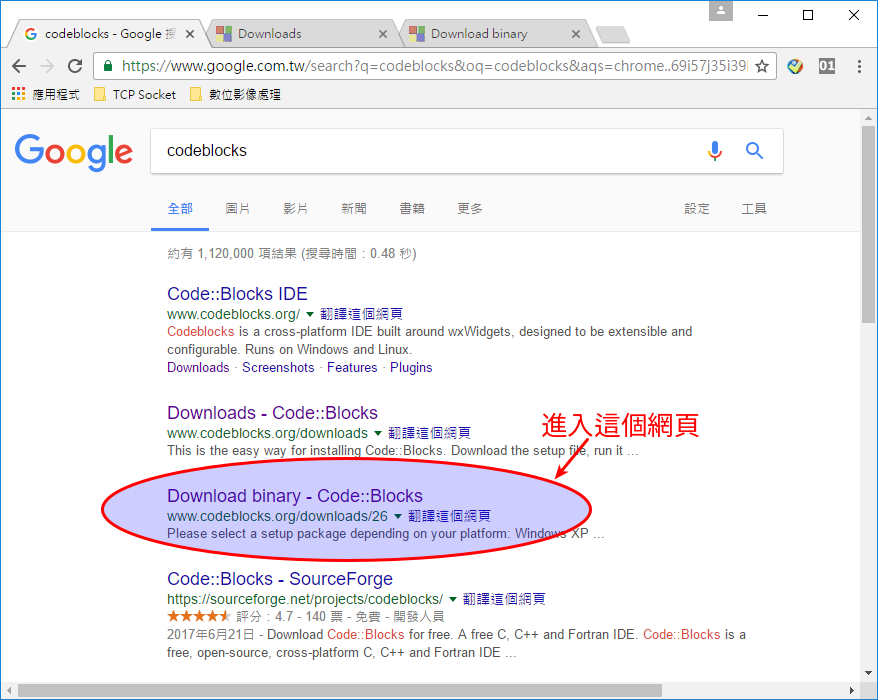
\includegraphics[width=0.8\textwidth]{fig/install_and_setting/install_001_searchCodeblocks}
		\caption{codeblocks搜尋結果}
		\label{install001}
	\end{figure}

	\begin{figure}[H]
		\centering
		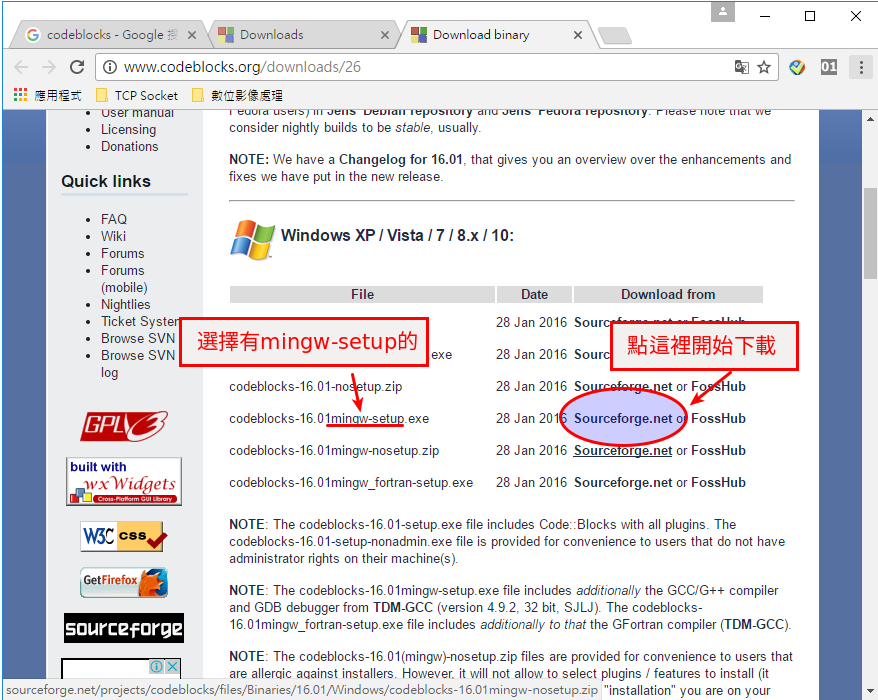
\includegraphics[width=0.8\textwidth]{fig/install_and_setting/install_002_Download_binary}
		\caption{Download binary頁面}
		\label{install002}
	\end{figure}
	
	找到剛剛下載的安裝檔codeblocks-16.01mingw-setup.exe,點兩下開啟安裝精靈,參考\autoref{install003}。
	\begin{figure}[H]
		\centering
		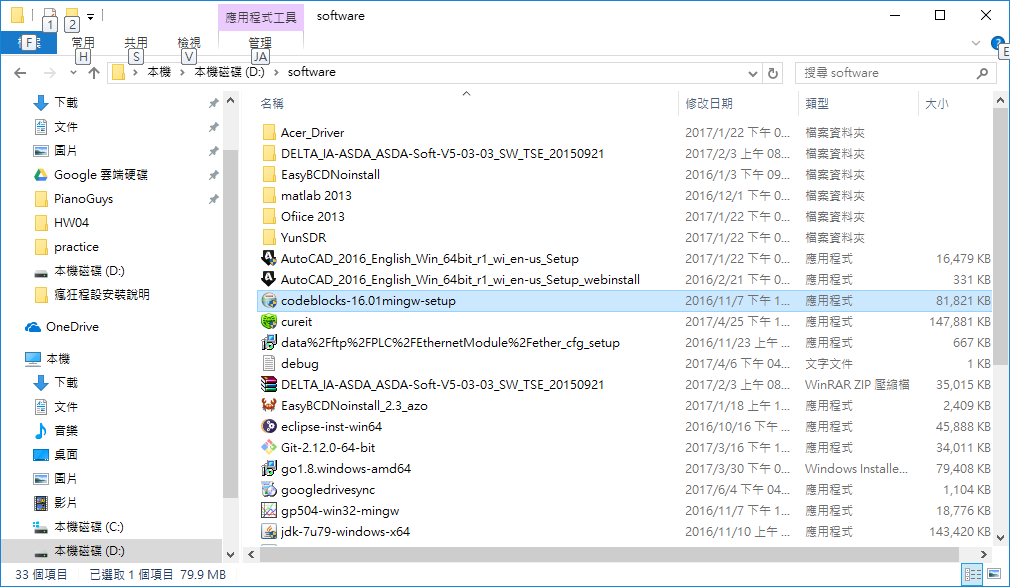
\includegraphics[width=0.8\textwidth]{fig/install_and_setting/install_003_openEXE}
		\caption{點兩下開啟CodeBlocks安裝檔}
		\label{install003}
	\end{figure}
	
	請不要修改安裝精靈的任何設定,只要一直點「Next」就好。絕對不可以更改檔案路徑,參考\autoref{install004}。
		\begin{figure}[H]
			\centering
			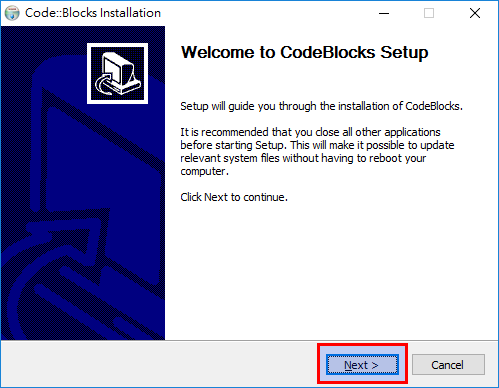
\includegraphics[width=0.8\textwidth]{fig/install_and_setting/install_004_setup01}
			\caption{啟動安裝精靈,點「Next」}
			\label{install004}
		\end{figure}
	
		\begin{figure}[H]
			\centering
			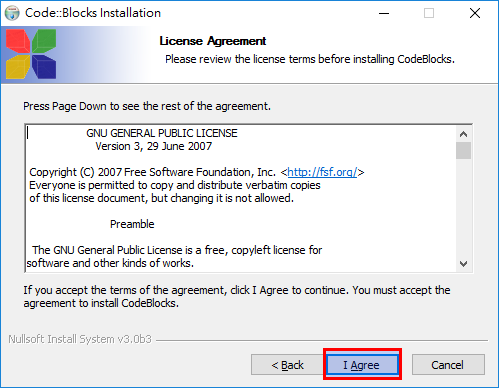
\includegraphics[width=0.8\textwidth]{fig/install_and_setting/install_005_setup02}
			\caption{點「I Agree」}
		\end{figure}
			
		\begin{figure}[H]
			\centering
			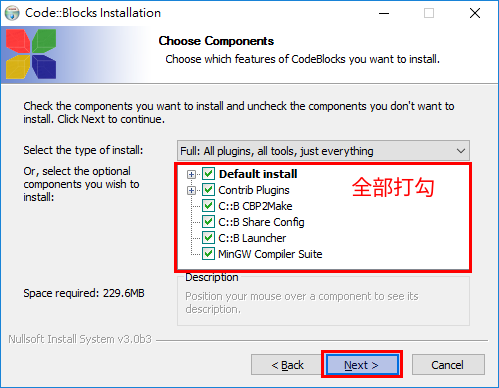
\includegraphics[width=0.8\textwidth]{fig/install_and_setting/install_006_setup03}
			\caption{全部打勾,點「Next」}
		\end{figure}
	
		\begin{figure}[H]
			\centering
			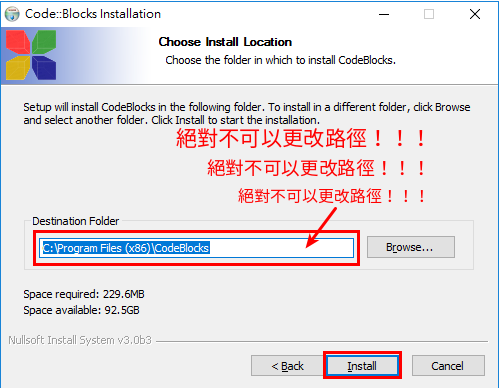
\includegraphics[width=0.8\textwidth]{fig/install_and_setting/install_007_setup04}
			\caption{直接點「Install」,絕對不可以更改路徑}
		\end{figure}

		\begin{figure}[H]
			\centering
			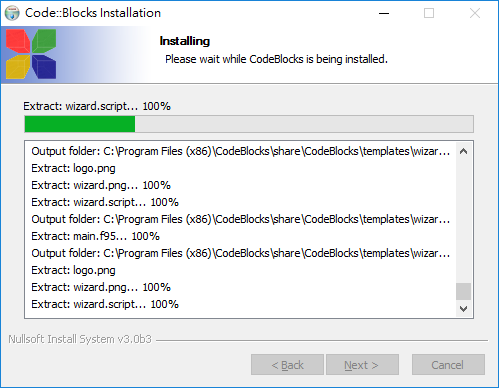
\includegraphics[width=0.8\textwidth]{fig/install_and_setting/install_008_setup05}
			\caption{正在安裝,請耐心等待}
		\end{figure}
		
		\begin{figure}[H]
			\centering
			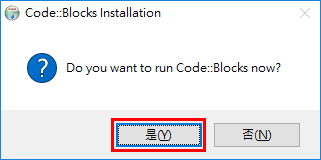
\includegraphics[width=0.5\textwidth]{fig/install_and_setting/install_009_setup06}
			\caption{點「是(Y)」,起動codeBlocks}
		\end{figure}
		
		\begin{figure}[H]
			\centering
			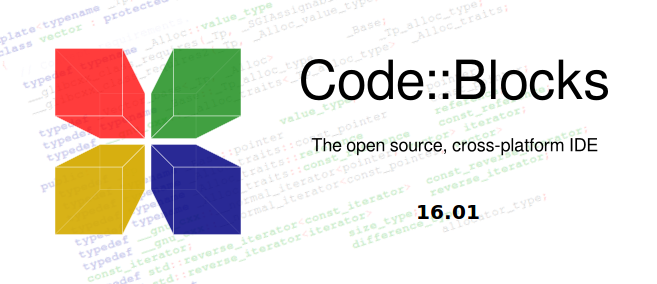
\includegraphics[width=0.8\textwidth]{fig/install_and_setting/install_010_setup07}
			\caption{正在開啟Codeblocks}
		\end{figure}
		
		\begin{figure}[H]
			\centering
			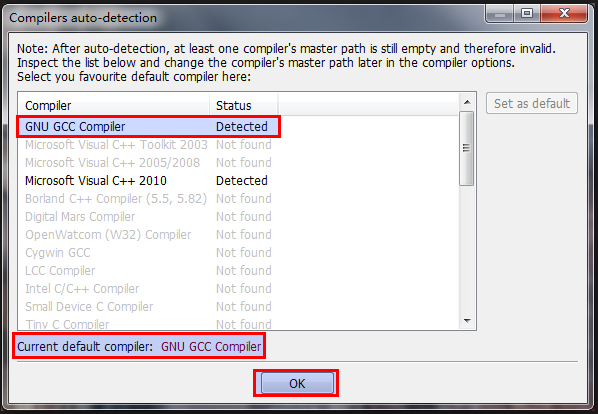
\includegraphics[width=0.8\textwidth]{fig/install_and_setting/install_011_setup08}
			\caption{確定有偵測到 GNU GCC Compiler,點「OK」}
		\end{figure}
		
		\begin{figure}[H]
			\centering
			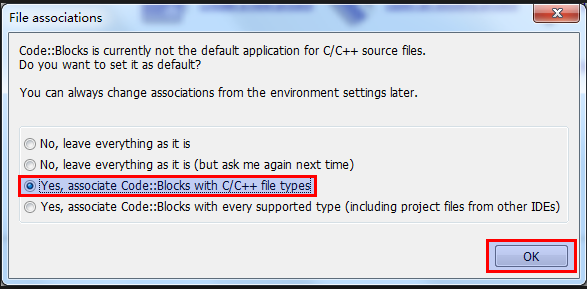
\includegraphics[width=0.8\textwidth]{fig/install_and_setting/install_012_setup09}
			\caption{選第三個,將CodeBlocks設為開啟程式碼的預設程式}
		\end{figure}
		
		\begin{figure}[H]
			\centering
			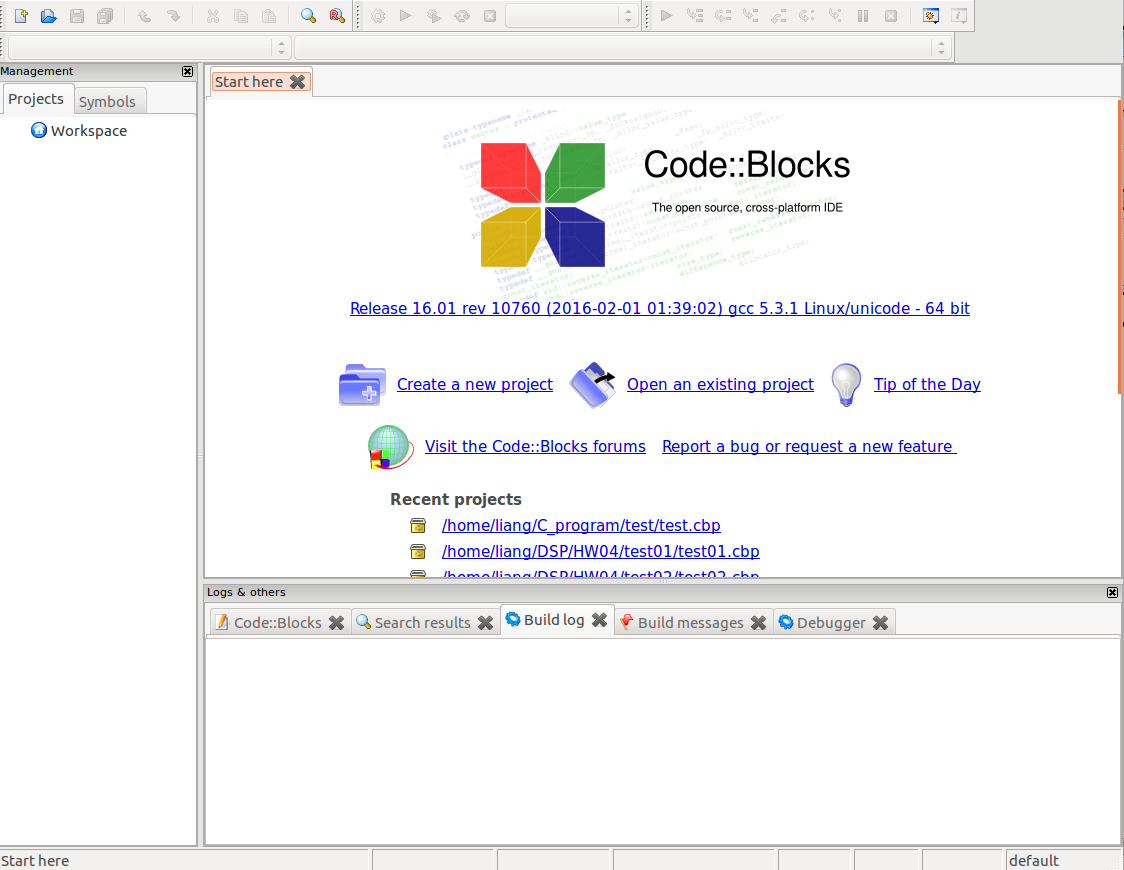
\includegraphics[width=0.8\textwidth]{fig/install_and_setting/install_013_setup10}
			\caption{成功開啟CodeBlocks}
		\end{figure}
		
		\begin{figure}[H]
			\centering
			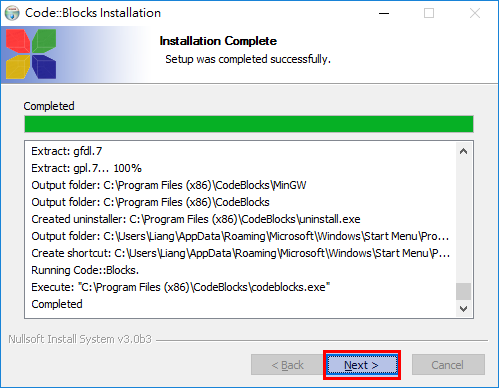
\includegraphics[width=0.8\textwidth]{fig/install_and_setting/install_014_setup11}
			\caption{回到安裝精靈,點「Next」}
		\end{figure}
		
		\begin{figure}[H]
			\centering
			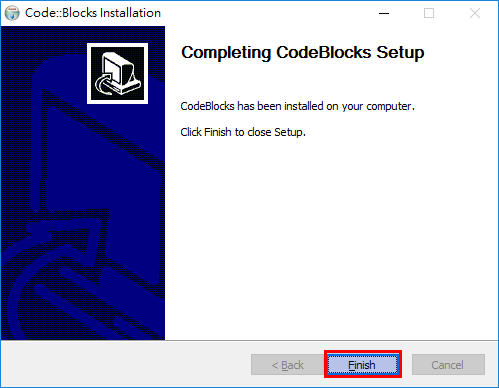
\includegraphics[width=0.8\textwidth]{fig/install_and_setting/install_015_setup12}
			\caption{點「Finish」,關閉安裝精靈}
		\end{figure}
	
\section{安裝「瘋狂程設」}
在google瀏覽器上搜尋關鍵字「瘋狂程設」,進入「瘋狂程設:自動閱卷的程式設計機上考試題庫暨考試系統」網站。也可以直接輸入網址:\url{http://coding-frenzy.arping.me/},參考\autoref{install016}。
		\begin{figure}[H]
			\centering
			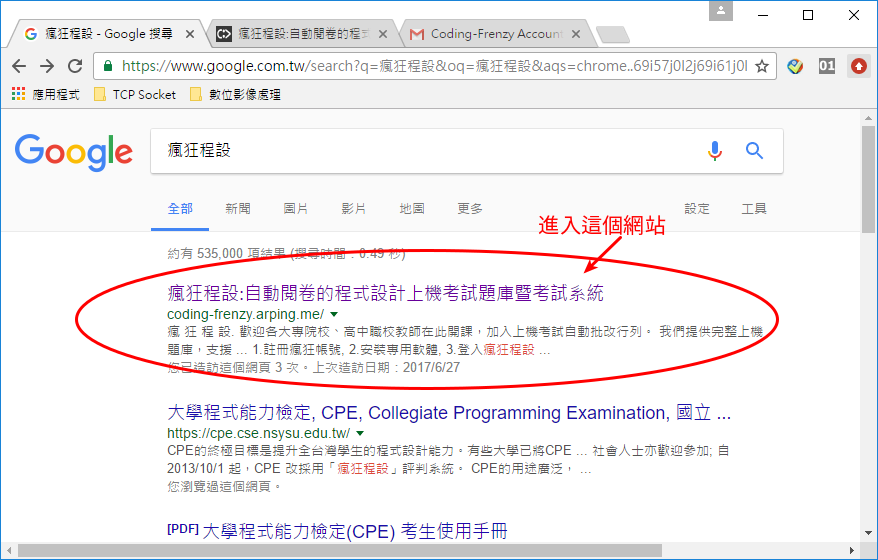
\includegraphics[width=0.8\textwidth]{fig/install_and_setting/install_016}
			\caption{「瘋狂程設」搜尋結果}
			\label{install016}
		\end{figure}
		進入瘋狂程設首頁後,點下方的「2.安裝專用軟體」,參考\autoref{install017}及\autoref{install018}。
		\begin{figure}[H]
			\centering
			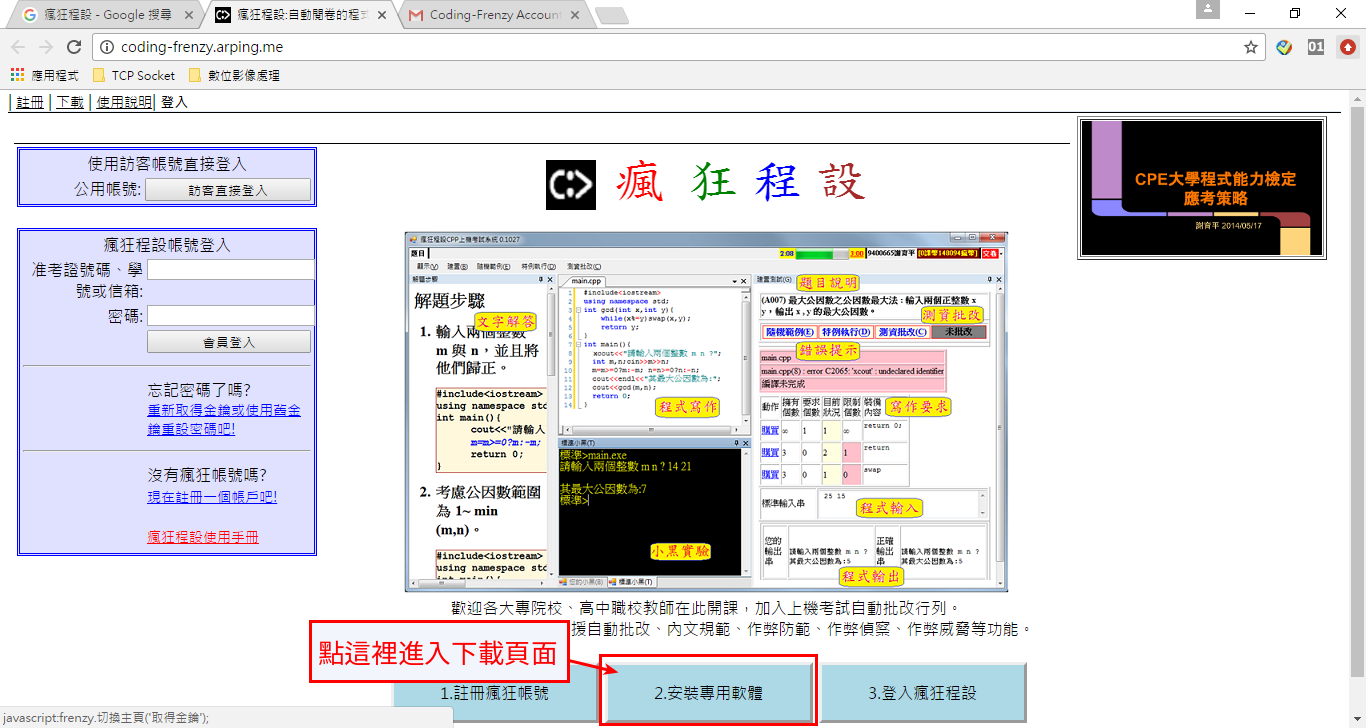
\includegraphics[width=0.9\textwidth]{fig/install_and_setting/install_017}
			\caption{瘋狂程設首頁}
			\label{install017}
		\end{figure}
		
		\begin{figure}[H]
			\centering
			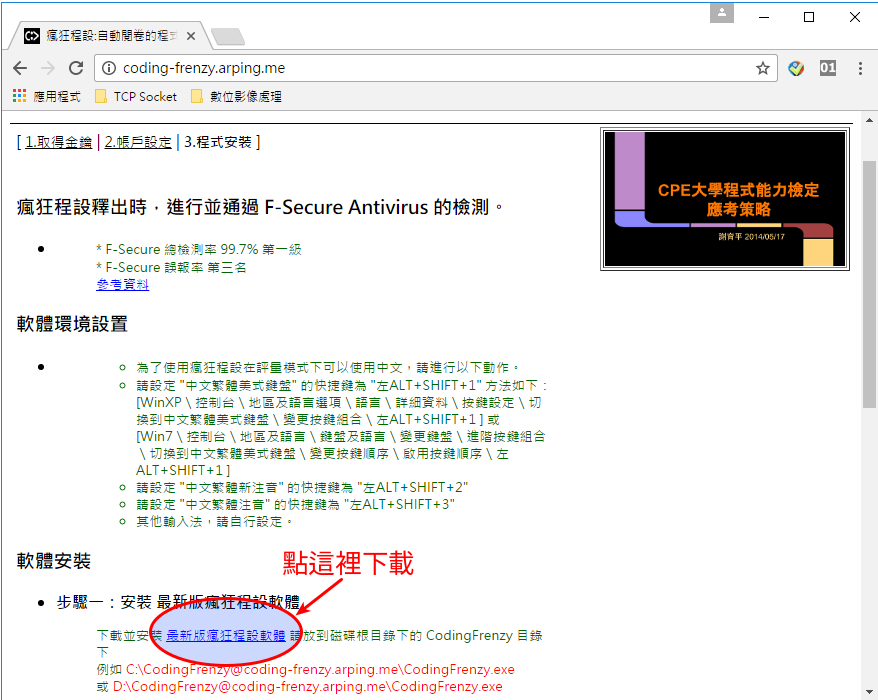
\includegraphics[width=0.9\textwidth]{fig/install_and_setting/install_018}
			\caption{下載頁面}
			\label{install018}
		\end{figure}
		
		 請將剛才下載的壓縮檔複製到C槽裡,直接放在根目錄C下面,然後解壓縮。對zip檔按「右鍵」 -> 解壓縮到CodingFrenzy@coding-frenzy.arping.me\textbackslash,參考\autoref{install019}。
		\begin{figure}[H]
			\centering
			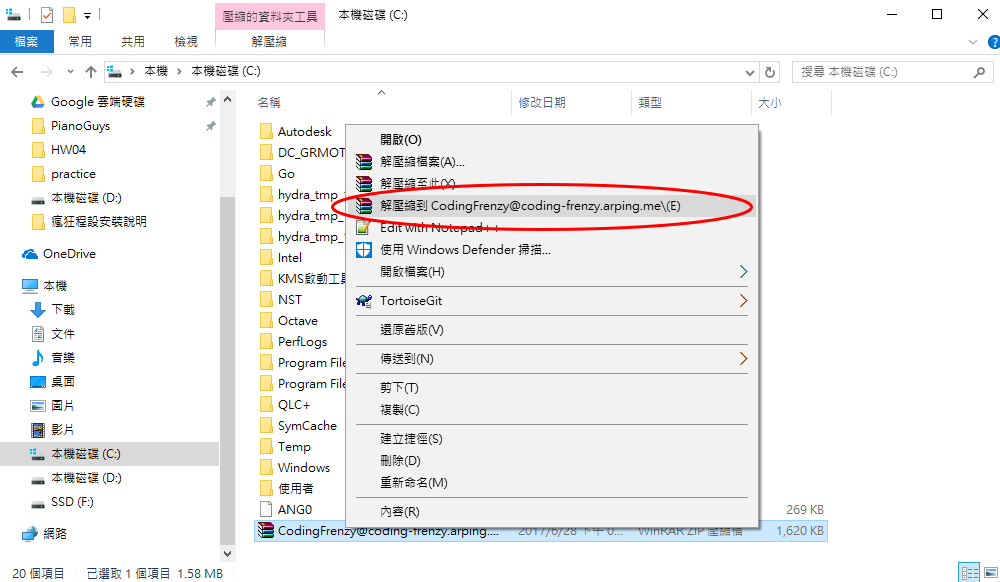
\includegraphics[width=0.95\textwidth]{fig/install_and_setting/install_019}
			\caption{右鍵 -> 解壓縮到CodingFrenzy@coding-frenzy.arping.me\textbackslash}
			\label{install019}
		\end{figure}

		之後,C槽裡面會出現一個資料夾「CodingFrenzy@coding-frenzy.arping.me」,點開此資料夾,參考\autoref{install020}。
		\begin{figure}[H]
			\centering
			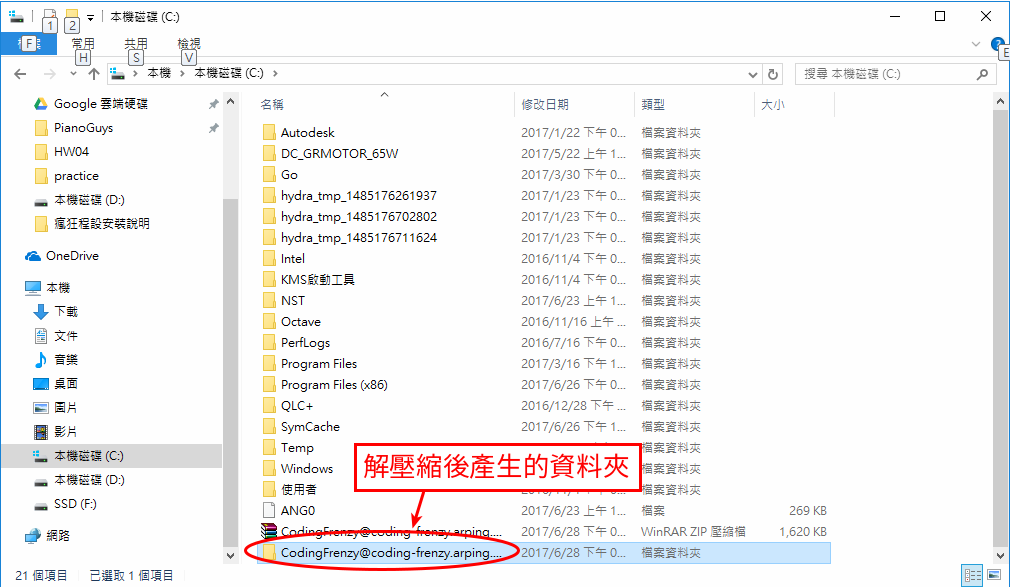
\includegraphics[width=\textwidth]{fig/install_and_setting/install_020}
			\caption{點開解壓縮後的資料夾}
			\label{install020}
		\end{figure}
		\begin{figure}[H]
			\centering
			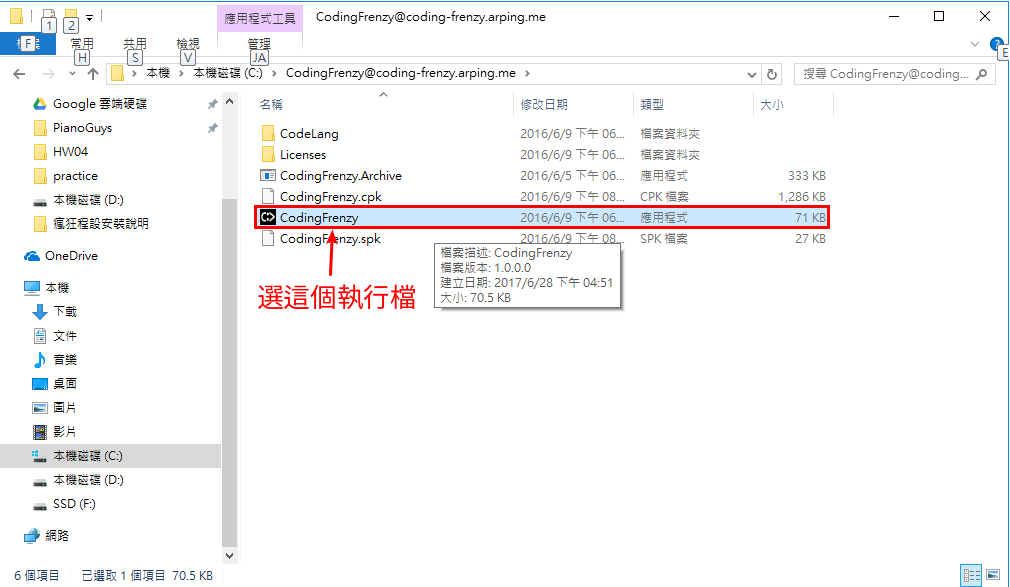
\includegraphics[width=\textwidth]{fig/install_and_setting/install_021}
			\caption{開啟CodingFrenzy執行檔}
		\end{figure}
		\begin{figure}[H]
			\centering
			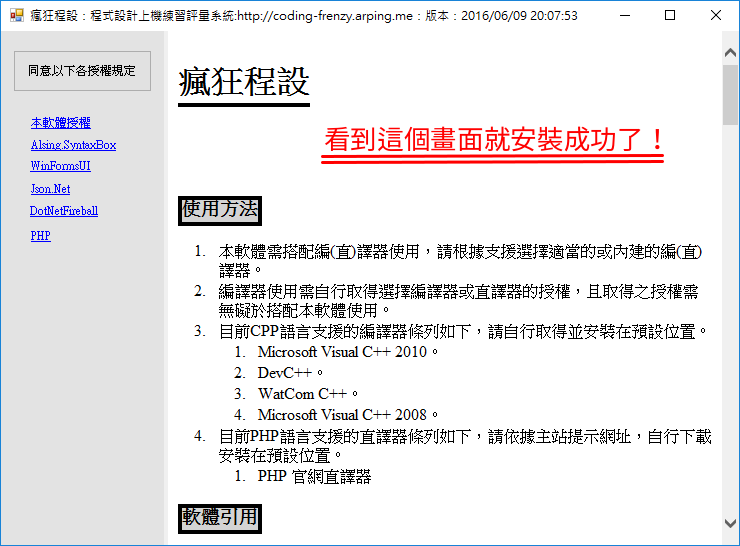
\includegraphics[width=0.8\textwidth]{fig/install_and_setting/install_022}
			\caption{安裝成功}
		\end{figure}

		回到資料夾裡,會多出一些東西,不用理它們。對CodingFrenzy.exe執行檔按「右鍵」-> 「傳送到」 -> 「桌面(建立捷徑)」,參考\autoref{install023}。
		\begin{figure}[H]
			\centering
			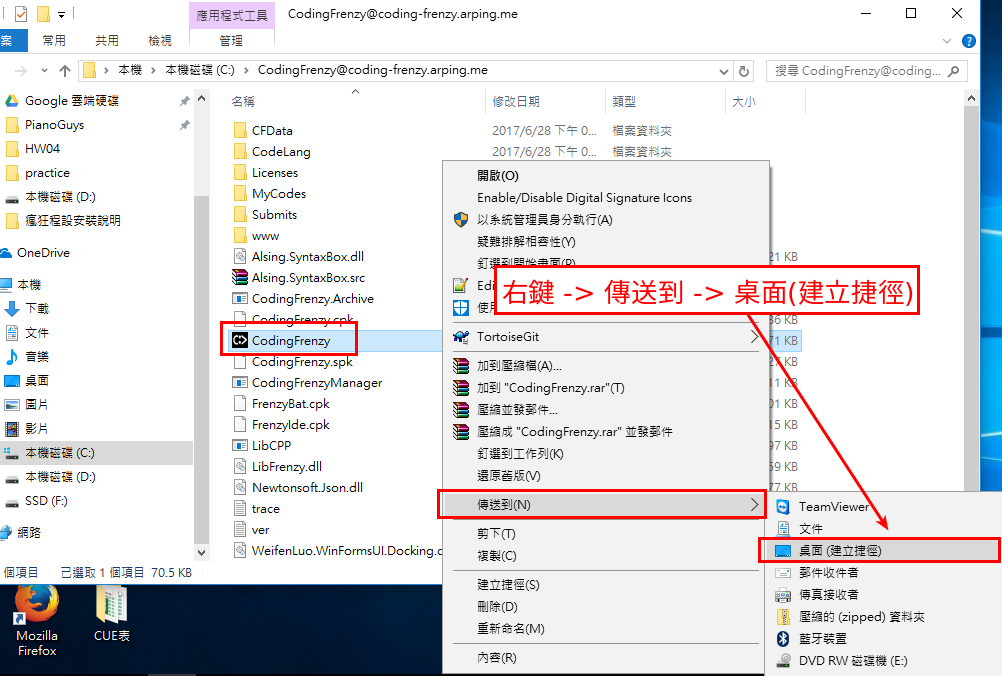
\includegraphics[width=\textwidth]{fig/install_and_setting/install_023}
			\caption{建立桌面捷徑}
			\label{install023}
		\end{figure}
	
		按鍵盤「win+D」切換到桌面,找到CodingFrenzy桌面捷徑,以後就可以從這邊直接執行瘋狂程設了,參考\autoref{install024}。
		\begin{figure}[H]
			\centering
			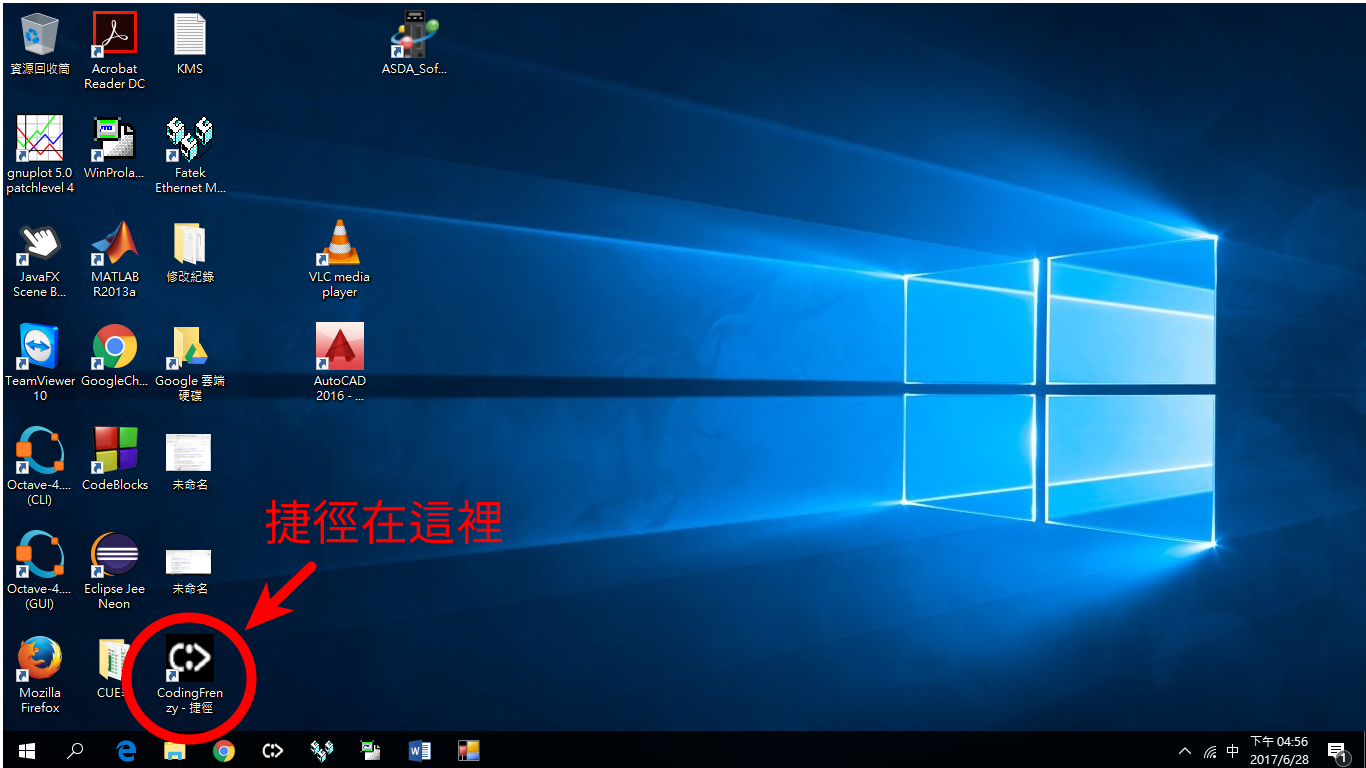
\includegraphics[width=0.9\textwidth]{fig/install_and_setting/install_024}
			\caption{桌面捷徑建立成功}
			\label{install024}
		\end{figure}

\section{註冊瘋狂程設的帳號}
現在要教同學如何註冊瘋狂程設的帳號。網頁版及桌面版的瘋狂程設皆可註冊,方法大同小異,範例是使用網頁版進行註冊。

進入\href{http://coding-frenzy.arping.me/}{「瘋狂程設」}首頁後,點選左下角的「現在註冊一個帳戶吧!」,參考\autoref{register001}。
\begin{figure}[H]
	\centering
	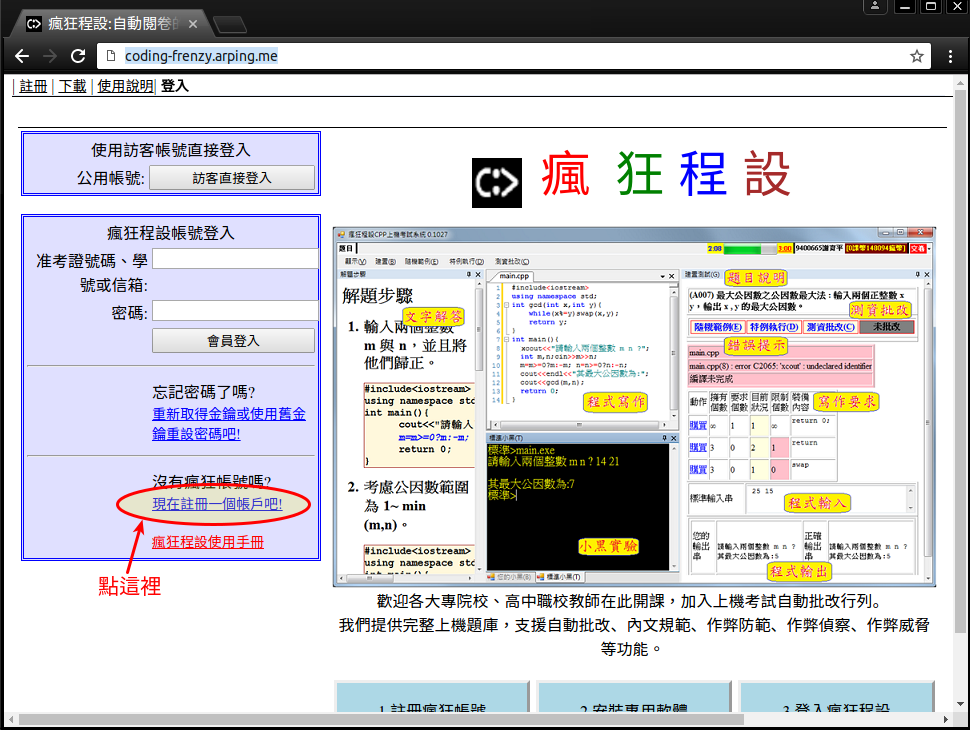
\includegraphics[width=0.8\textwidth]{fig/install_and_setting/register_001}
	\caption{註冊新帳戶}
	\label{register001}
\end{figure}

在框框處輸入你的電子信箱,完成後,按下方的按鈕「取得帳號金鑰」,參考\autoref{register002}。
\begin{figure}[H]
	\centering
	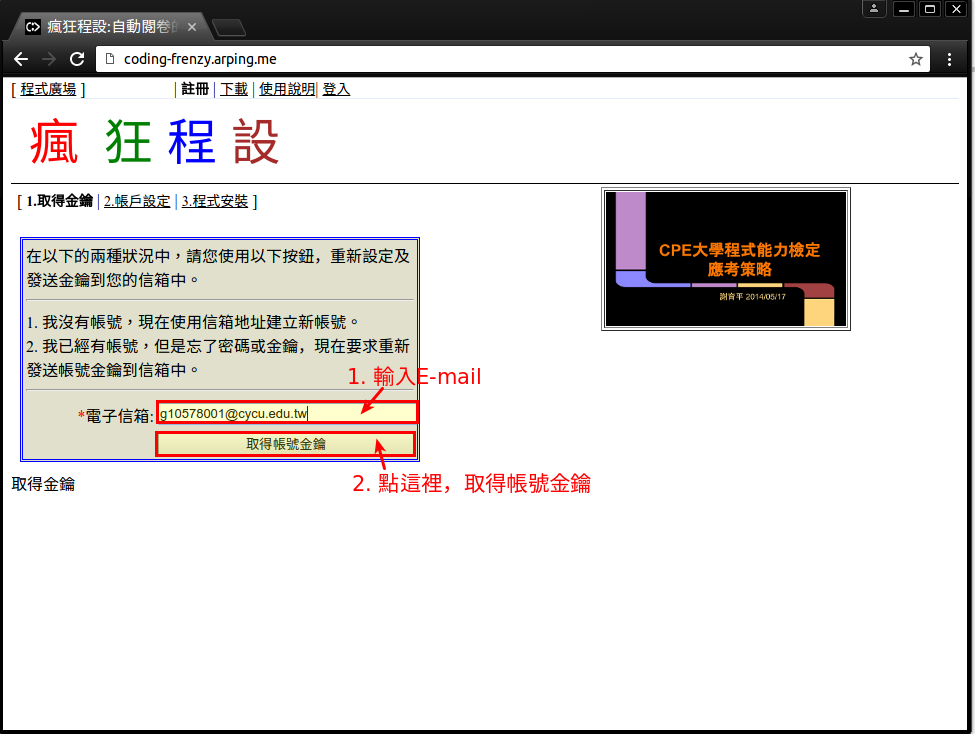
\includegraphics[width=0.8\textwidth]{fig/install_and_setting/register_002}
	\caption{輸入e-mail,取得金鑰}
	\label{register002}
\end{figure}


註冊成功會顯示紅字「註冊成功,請前往信箱提取開頭為xxxx的金鑰來設定密碼。」參考\autoref{register003}。※範例中的金鑰開頭四碼是e017,你的金鑰開頭四碼與範例不同是正常的。
\begin{figure}[H]
	\centering
	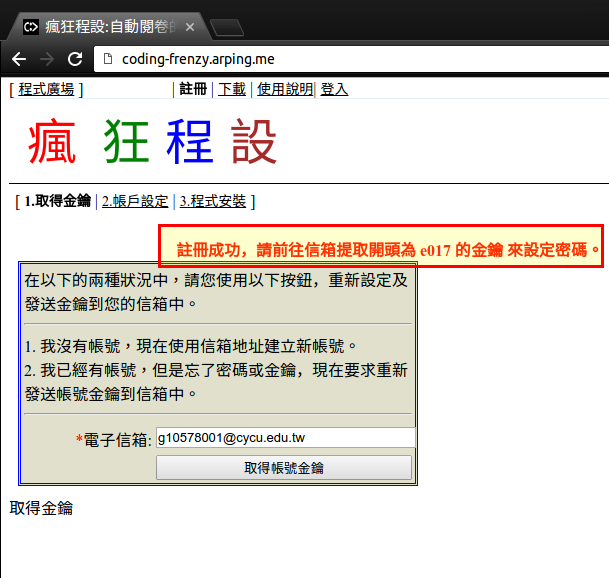
\includegraphics[width=0.6\textwidth]{fig/install_and_setting/register_003}
	\caption{成功取得金鑰}
	\label{register003}
\end{figure}

到你的電子信箱去收信,會收到一封主旨為「Coding-Frenzy Account is Created」的信,若沒收到可以去垃圾信件夾找找看,參考\autoref{register004}。
\begin{figure}[H]
	\centering
	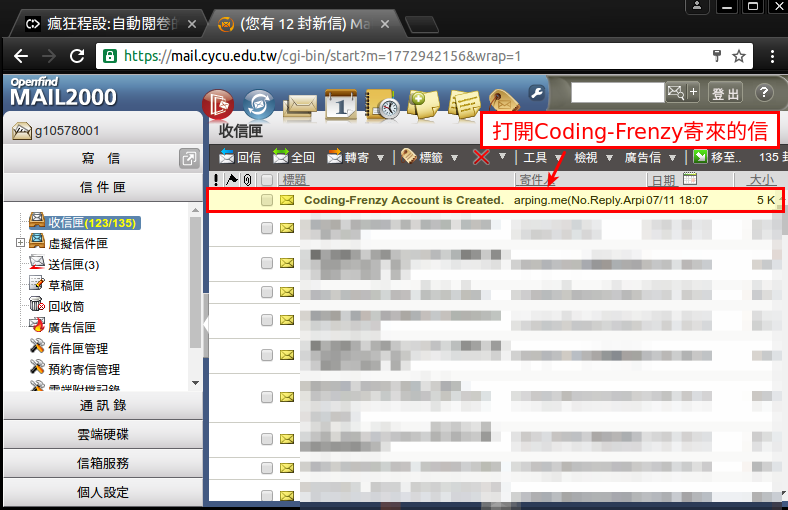
\includegraphics[width=0.8\textwidth]{fig/install_and_setting/register_004}
	\caption{去你的電子信箱收信}
	\label{register004}
\end{figure}

點LINK後面的連結,會自動開啟一個新的分頁,進入「帳戶設定」頁面,參考\autoref{register005}。
\begin{figure}[H]
	\centering
	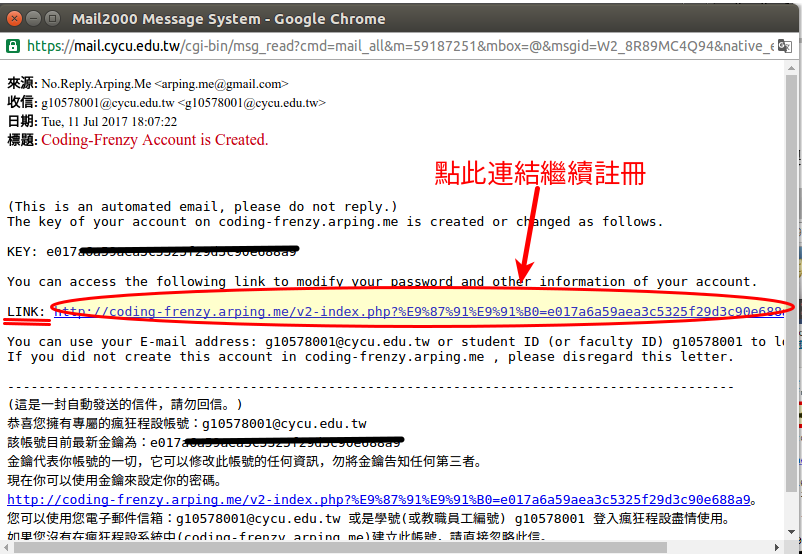
\includegraphics[width=0.8\textwidth]{fig/install_and_setting/register_005}
	\caption{點LINK後面的連結}
	\label{register005}
\end{figure}

\newpage
系統會自動填寫金鑰,將個人資料填寫完畢後,按下「我同意修改資料,並放棄個資法的求償權利。」,參考\autoref{register006}。

\begin{figure}[H]
	\centering
	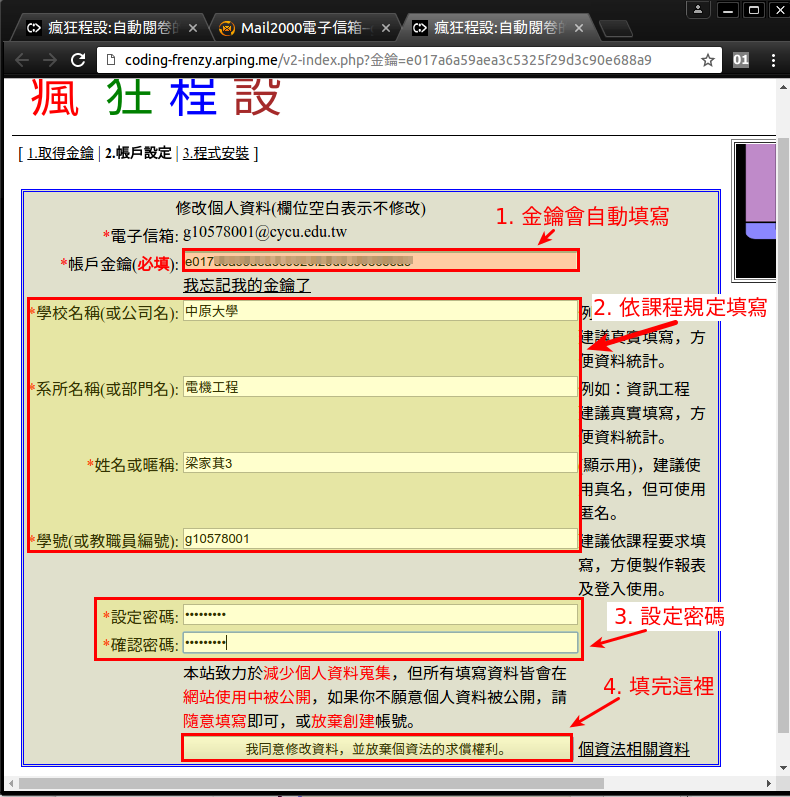
\includegraphics[width=0.9\textwidth]{fig/install_and_setting/register_006}
	\caption{填寫基本資料}
	\label{register006}
\end{figure}

\newpage
按下按鈕後,畫面沒有變化是正常的,這時候請先「登出」(頁面上方),參考\autoref{register007}。
\begin{figure}[H]
	\centering
	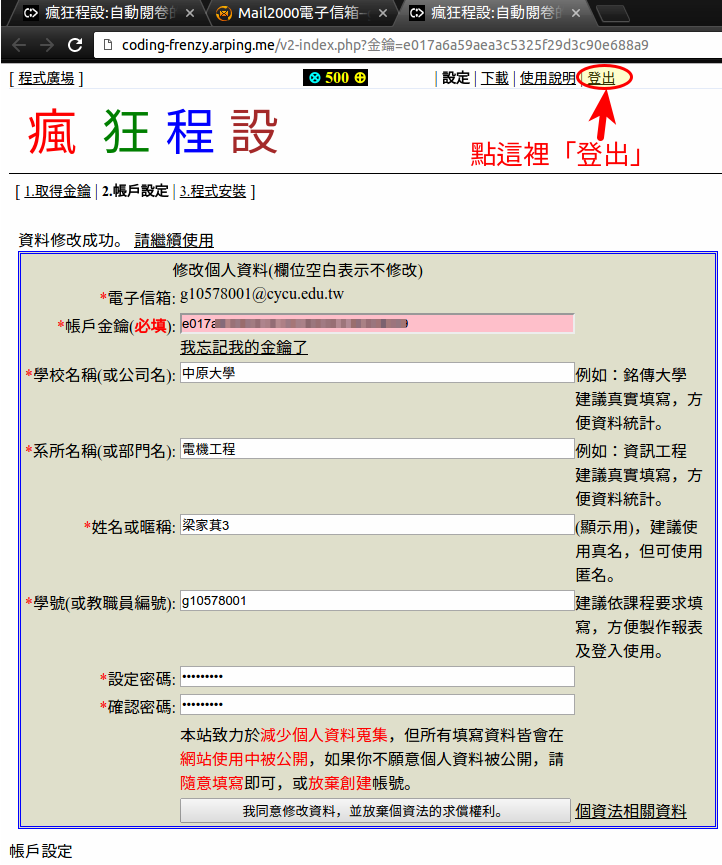
\includegraphics[width=0.9\textwidth]{fig/install_and_setting/register_007}
	\caption{登出}
	\label{register007}
\end{figure}

\newpage
回到首頁後,用剛剛設定的學號及密碼登入,參考\autoref{register008}。


\begin{figure}[H]
	\centering
	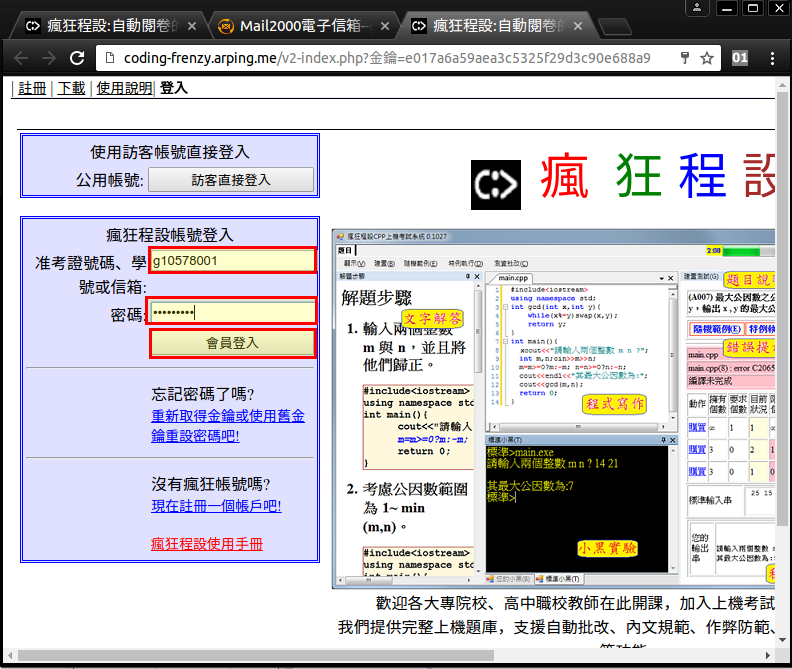
\includegraphics[width=0.9\textwidth]{fig/install_and_setting/register_008}
	\caption{登入畫面}
	\label{register008}
\end{figure}

\newpage
若看到此畫面,恭喜你完成註冊,參考\autoref{register009}。

\begin{figure}[H]
	\centering
	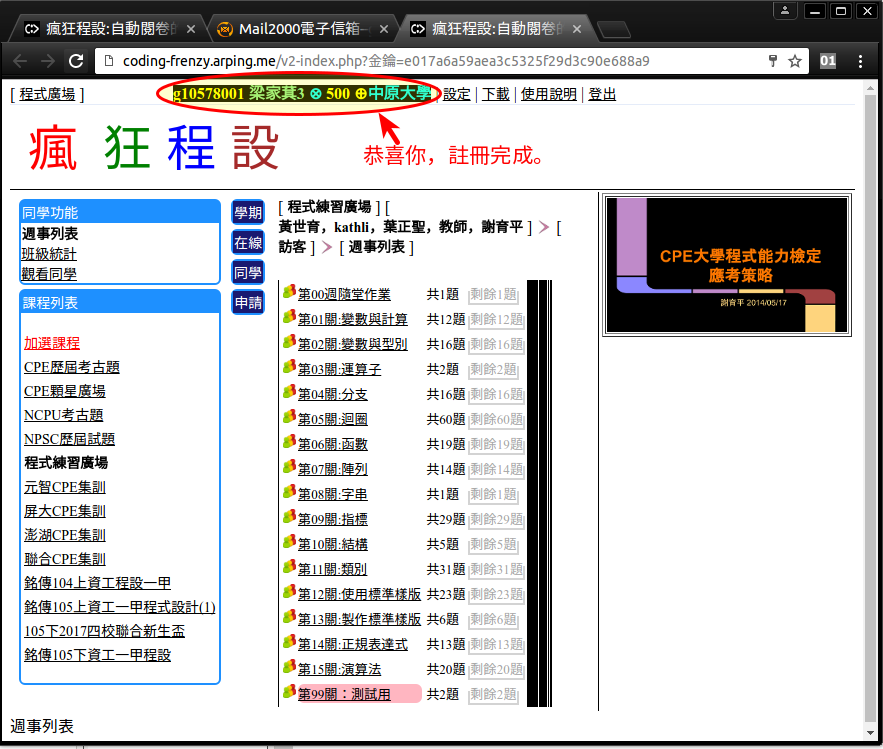
\includegraphics[width=0.9\textwidth]{fig/install_and_setting/register_009}
	\caption{登入成功}
	\label{register009}
\end{figure}

\section{如何使用瘋狂程設}
現在要說明如何使用瘋狂程設練習寫程式。

\begin{enumerate}
\item 點擊「程式練習廣場」。
\item 點擊「第01關:變數與計算」。
\item 點擊「練習」A001:Hello World。

參考\autoref{use001}。
\begin{figure}[H]
	\centering
	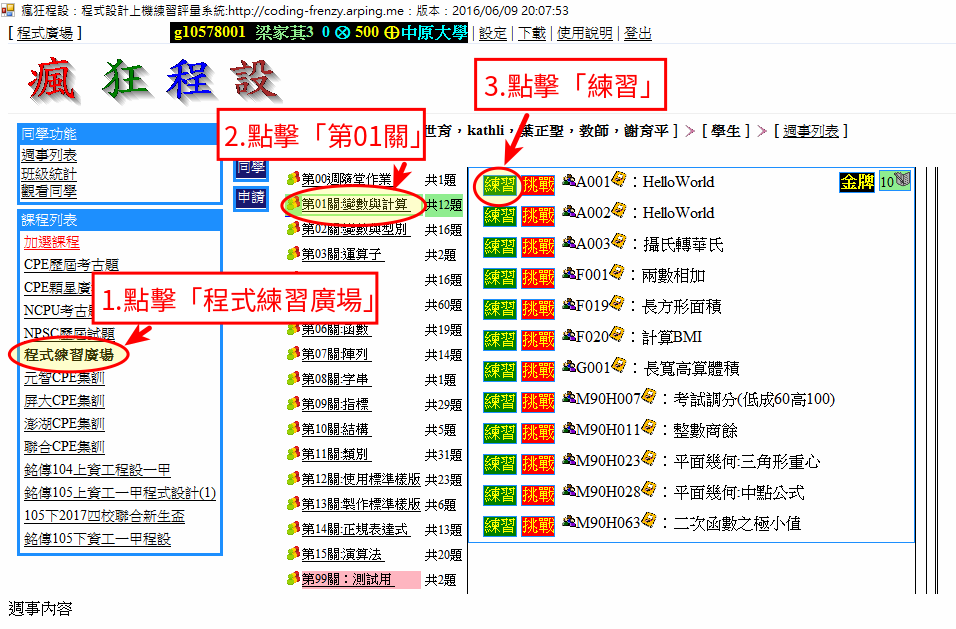
\includegraphics[width=0.9\textwidth]{fig/install_and_setting/use_001}
	\caption{選擇練習題目}
	\label{use001}
\end{figure}


\item 查看「題目資料」。
\item 有些題目的「解文」會有解題步驟。
\item 輸入程式碼。

注:程式碼的解說會在後續章節詳細說明,現在請直接照圖片上的範例輸入程式碼,或是複製「解文」裡的程式碼。

參考\autoref{use002}。
\begin{figure}[H]
	\centering
	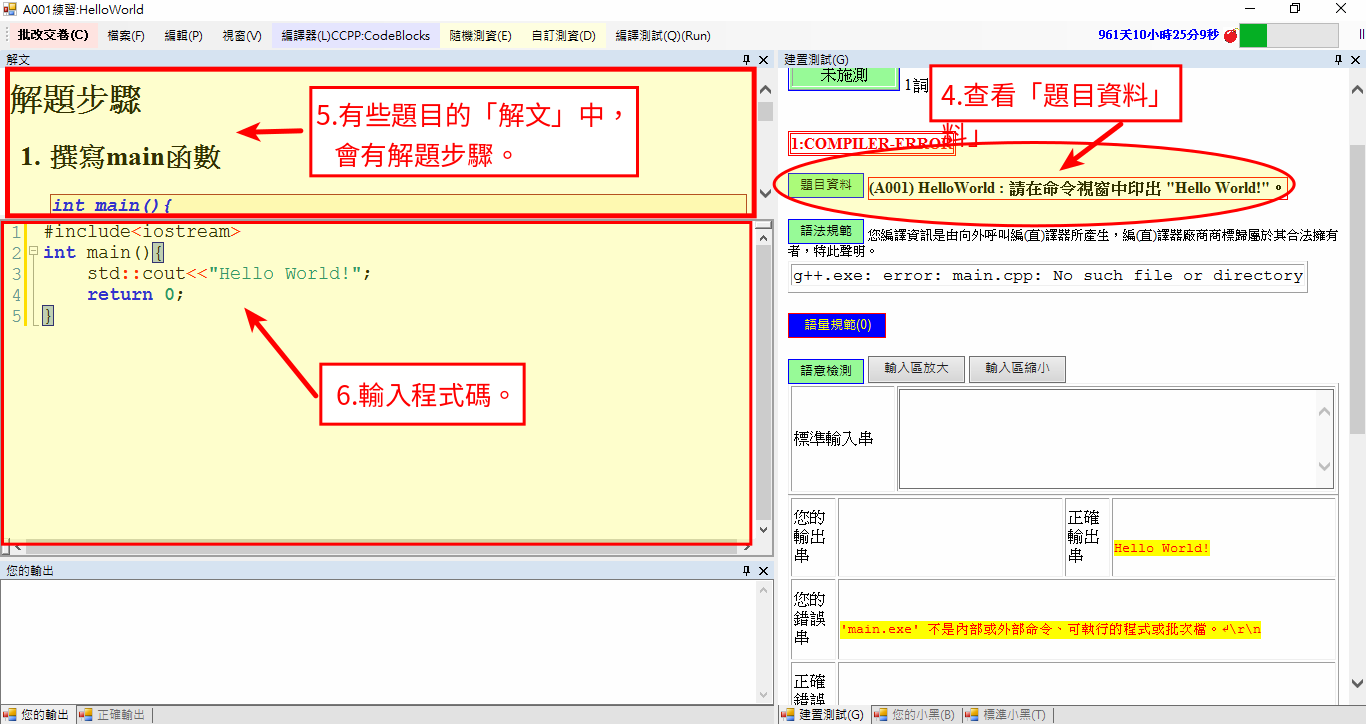
\includegraphics[width=0.9\textwidth]{fig/install_and_setting/use_002}
	\caption{依題目要求輸入程式碼}
	\label{use002}
\end{figure}

\newpage
\item 設定「編譯器」,選擇「CCPP:CodeBlocks」,如果找不到此編譯器,請重新安裝CodeBlocks。

參考\autoref{use003}。
\begin{figure}[H]
	\centering
	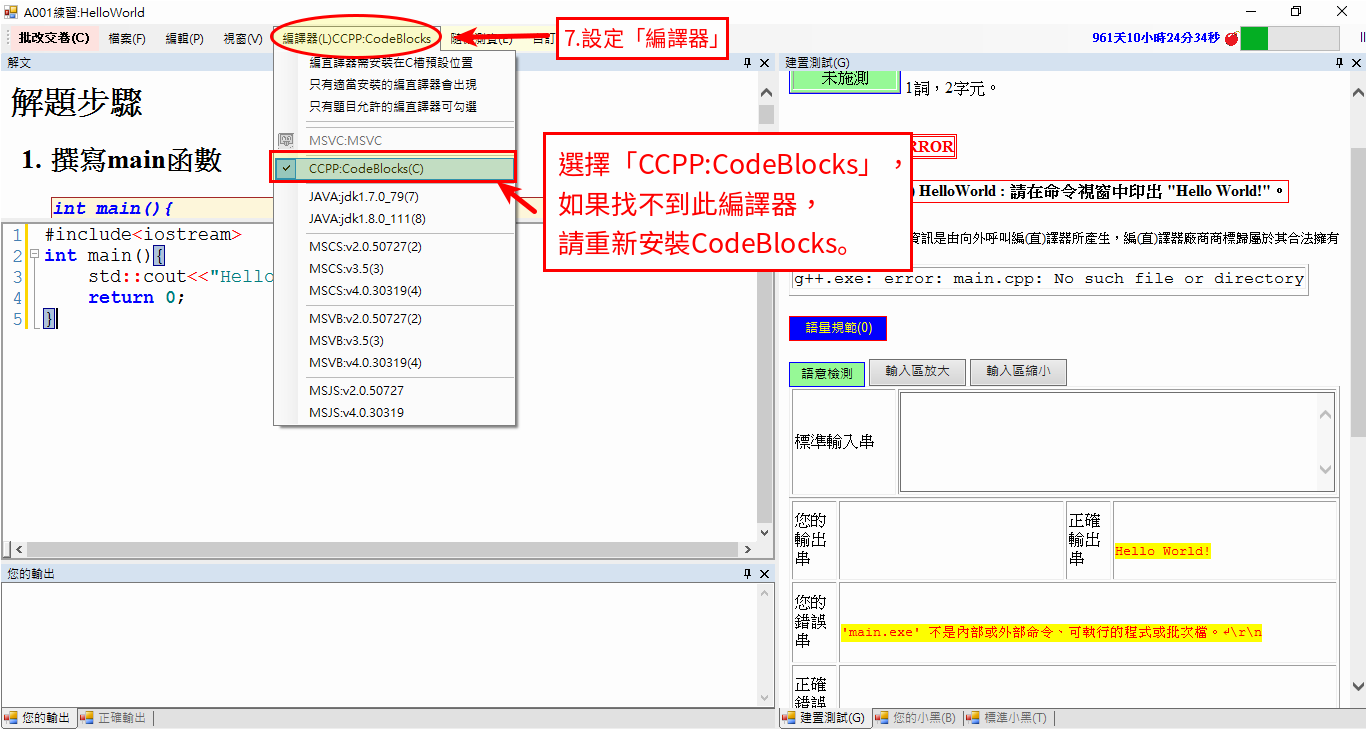
\includegraphics[width=0.8\textwidth]{fig/install_and_setting/use_003}
	\caption{設定「編譯器」}
	\label{use003}
\end{figure}


\item 點擊「隨機測資」或「自訂測資」。
\item 如果程式有錯誤。
\item 查看「編譯錯誤訊息」。

參考\autoref{use004}。
\begin{figure}[H]
	\centering
	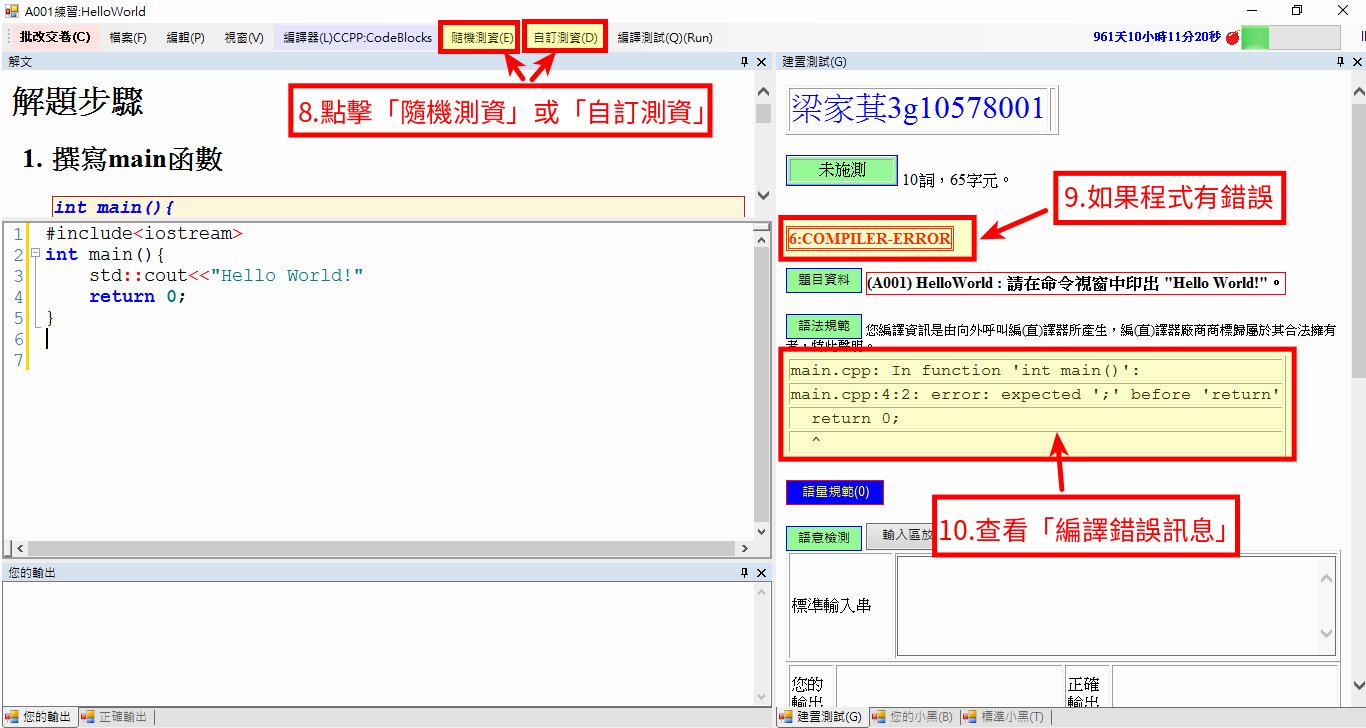
\includegraphics[width=0.8\textwidth]{fig/install_and_setting/use_004}
	\caption{測試程式碼}
	\label{use004}
\end{figure}


\item 修改程式碼。
\item 再次使用測資測試。
\item 程式正確,「顯示CORRECT」。
\item 點擊「批改交卷」。
\item 點擊「確定」,關閉提示視窗。
\item 顯示「通過」。
\item 關閉作答視窗。

參考\autoref{use005}。
\begin{figure}[H]
	\centering
	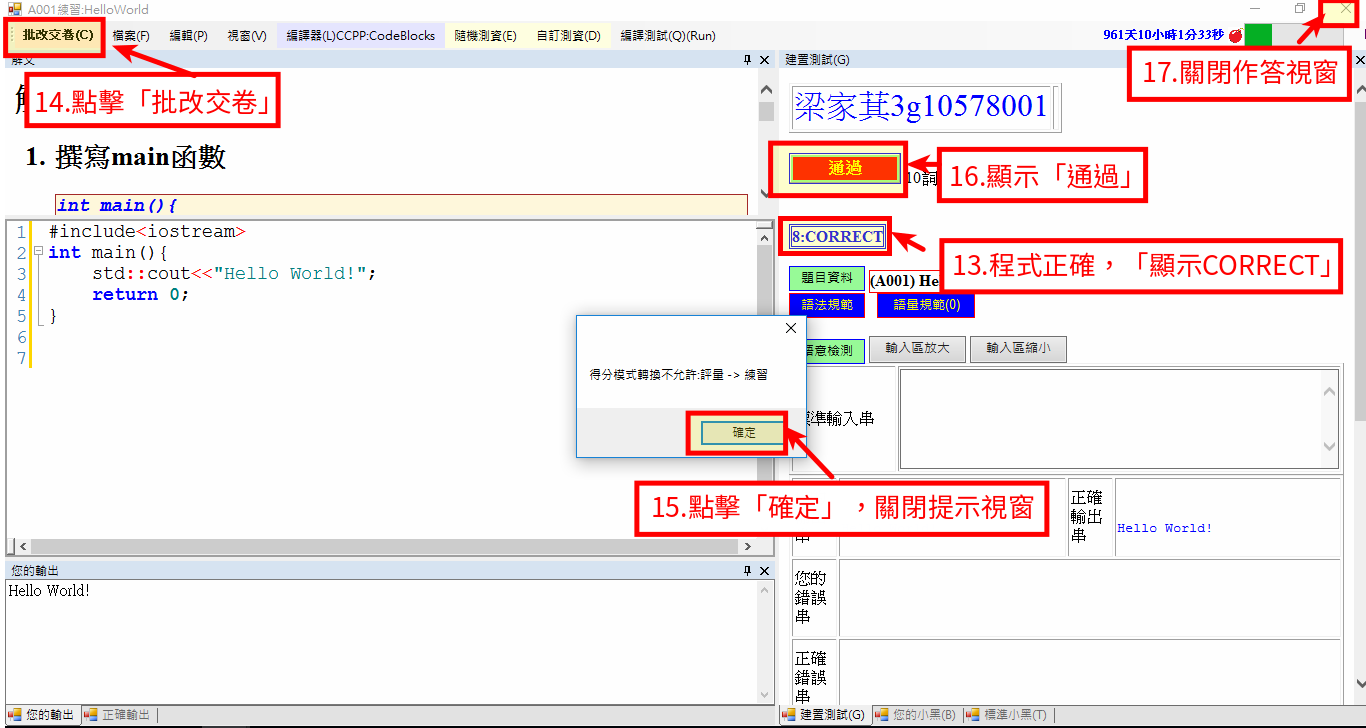
\includegraphics[width=0.8\textwidth]{fig/install_and_setting/use_005}
	\caption{批改交卷}
	\label{use005}
\end{figure}


\item 在主畫面按【F5】更新作答成績。
\item 通過「挑戰」模式,顯示「金牌」。
\item 通過「練習」模式,顯示「練習」。

參考\autoref{use006}。
\begin{figure}[H]
	\centering
	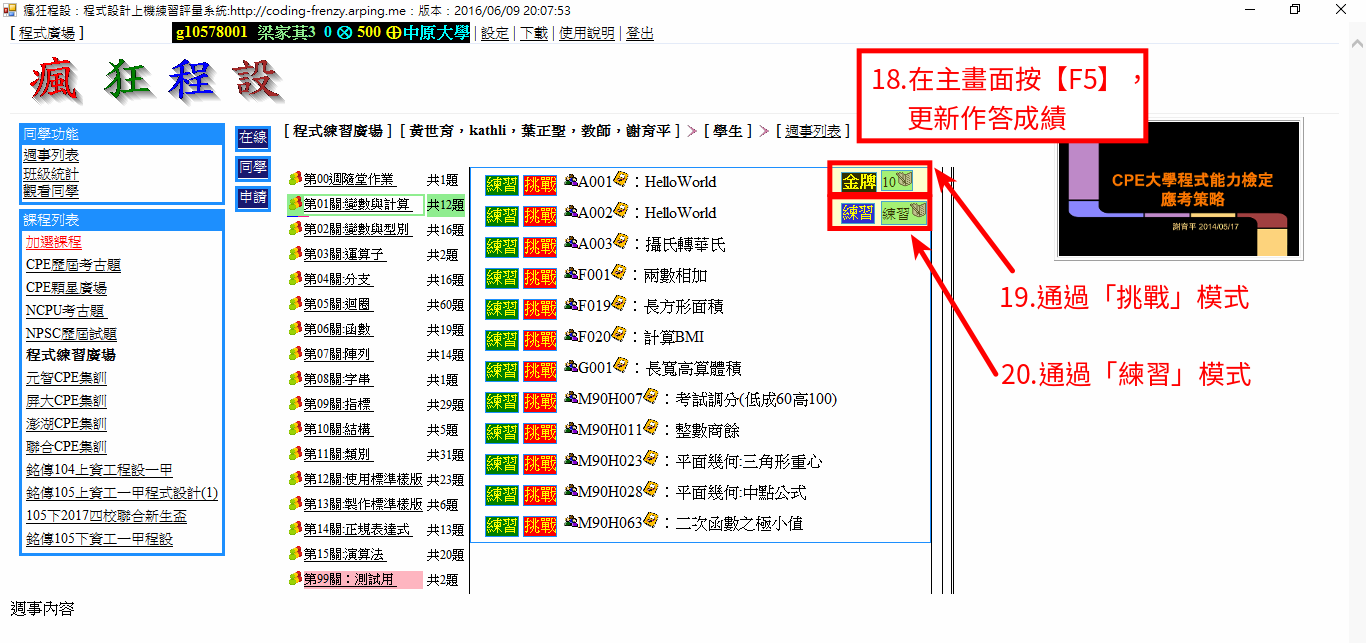
\includegraphics[width=0.9\textwidth]{fig/install_and_setting/use_006}
	\caption{查看成績}
	\label{use006}
\end{figure}

\end{enumerate}

\section{附錄二、輸入/輸出 (Input/Output, I/O)}
基本上,\cc{}語言涵括了C語言的功能,所以我們也可以在\cc{}的環境中,撰寫C的程式碼。一般而言,大部份的程式都會有輸入和輸出的需求,而\cc{}和C的輸入和輸出方式,各有其優點,在不同的場合,有時候使用\cc{}的輸入輸出方式會比較方便,有時候使用C的輸入輸出函數會比較方便,如果可以把兩種方式都學會,在撰寫程式碼的時候,可以有很多便利,所以這裡先介紹兩種語言基本的輸入和輸出的使用方法。

\subsection{C語言的輸入和輸出}
C語言使用scanf和printf兩個函數來做輸入和輸出,使用C語言的輸入輸出函數,C程式碼必須引入檔頭<stdio.h>,如果在\cc{}的環境中,則可以引入<stdio.h>或<cstdio>。以下先介紹printf函數的用法,接著再介紹scanf函數的用法。

\subsubsection {printf輸出函數}
C語言使用printf函數將訊息列印至標準輸出(standard output),一般而言,標準輸出指的是螢幕,除了列印字串,也可以列印各種型態的變數,執行過後會回傳所列印的字元數。printf函數至少要有一個參數,而且第一個參數一定是一個字串,執行結果會把這個字串列印到螢幕上,例如:
\begin{inside}
	printf("format string");
\end{inside}
其執行結果如下:
\begin{Verbatim}
    format string
\end{Verbatim}
字串中可以加入跳脫符號,用來控制輸出的樣貌,常用的控制字元如\autoref{escapechar}所示,例如
$\backslash$n代表換行字元,如果希望在字串的某個地方換行,可以把$\backslash$n插入到字串裡面。

另外也可以在第一個字串中加上格式指定字元(format specifier),用來指明要列印的變數或數值型式,字串中有幾個格式指定字元,後面就必須加上相對應個數的參數,執行結果會先把各參數依指定型式放到字串中,然後再將字串輸出。常見的格式指定字元如\autoref{specifier}所示。

\begin{table}[H]
\centering
\caption{字串中常用的跳脫符號}
\begin{tabular}{|c|l|}
	\hline
	\rowcolor{LightCyan}
	字元格式 & 字元功能\\
	\hline
	\textbackslash 0& 空格\\
	\hline
	\textbackslash b& 倒退\\
	\hline
	\textbackslash t&移到下一定位,即【Tab】鍵。\\
	\hline
	\textbackslash n&游標移到下一列。\\
	\hline
	\textbackslash "&插入雙引號。\\
	\hline
	\textbackslash '&插入單引號。\\
	\hline
	\textbackslash \textbackslash&插入反斜線。\\
	\hline
	\textbackslash a &發出警告聲。\\
	\hline
\end{tabular}
\label{escapechar}
\end{table}

\begin{table}[H]
\centering
\caption{printf常見的格式指定字元}
\begin{tabular}{|l|l|}
	\hline
	\rowcolor{LightCyan}
	指定碼格式 & 功能\\
	\hline
	\%c& 以字元方式輸出。 \\
	\hline
	\%d&  	10 進位整數輸出。\\
	\hline
	\%o& 	以 8 進位整數方式輸出。\\
	\hline
	\%u&  	無號整數輸出。\\
	\hline
	\%x,\%X &	將整數以 16 進位方式輸出 。\\
	\hline
	\%f&  浮點數輸出。\\
	\hline
	\%e,\% E& 	使用科學記號顯示浮點數 。\\
	\hline
	\%g,\%G &浮點數輸出,取 \%f 或 \%e(\%f 或 \%E),看哪個表示精簡。\\
	\hline
	\%\% &顯示。 \%\\
	\hline
	\%s & 	字串輸出。 \\
	\hline
	\%lu &long unsigned 型態的整數。\\
	\hline
	\%p &指標型態。\\
	\hline
\end{tabular}
\label{specifier}
\end{table}

舉例而言,
\begin{inside}
	var1 = 5;
	printf("The value of a and b = %d %f", var1, 3.14159);
\end{inside}
其中\%d代表要放一個整數,\%f代表要放一個浮點數,這兩個數分別會從後面的var1及3.14159取得,其執行結果如下:
\begin{Verbatim}
	The value of a and b = 5 and 3.14159
\end{Verbatim}

以下是使用一些格式指定字元的範例程式碼:
\begin{cppcode}
#include <stdio.h>

int main() 
{
	printf("顯示字元 %c\n", 'A');
	printf("顯示字元編碼 %d\n", 'A');
	printf("顯示字元編碼 %c\n", 65);    
	printf("顯示十進位整數 %d\n", 15);
	printf("顯示八進位整數 %o\n", 15);
	printf("顯示十六進位整數 %X\n", 15);
	printf("顯示十六進位整數 %x\n", 15);    
	printf("顯示科學記號 %E\n", 0.001234);    
	printf("顯示科學記號 %e\n", 0.001234);    
	return 0;
}
\end{cppcode}
上述程式碼的執行結果:
\begin{figure}[H]
	\centering
	\includegraphics[width=17cm]{fig/cpp_io/HW007}
\end{figure}

\subsubsection {scanf輸入指令}
C語言使用scanf函數從標準輸入(standard input)來讀取變數的值,一般而言,標準輸入指的是鍵盤。scanf的第一個參數是一個字串,通常裡面都放格式指定字元和空白,表示要讀入的變數的型態,後面必須加上與格式指定字元同樣個數及相應型態的變數,並且在變數前要加上\&字元,以下是一個簡單的範例:
\begin{cppcode}
#include <stdio.h>

int main() {
	int input;
	printf("請輸入數字:");
	scanf("%d", &input);
	printf("您輸入的數字:%d\n", input);
	return 0;
}
\end{cppcode}
其執行結果如下:
\begin{figure}[H]
	\includegraphics[width=17cm]{fig/cpp_io/HW008}
\end{figure}


\subsection{\cc{}語言的輸入和輸出}
\cc{}語言使用cin和cout來做輸入和輸出,使用\cc{}語言的輸入輸出,程式碼必須引入檔頭<iostream>。另外\cc{}有所謂的命名空間,所有標準輸入和輸出相關的函數、指令和參數等,都定義在std的命名空間中,使用這些函數、指令或參數的時候,必須在前面加上std::,例如使用cout的時候,必須寫成std::cout,如果覺得這樣很麻煩,可以在引入檔頭之後,加上以下指令
\begin{inside}
	using namespace std;
\end{inside}
代表要引入std命名空間中的所有函數、指令和參數等,這樣就可以直接使用cout等指令,不用再加上std::的前綴。

以下先介紹cout的用法,接著再介紹cin的用法。

\subsubsection{cout輸出指令}
\cc{}語言使用cout指令將資料送到標準輸出,若沒有特別設定,會由電腦螢幕上顯示。使用方式以範例說明如下:
\begin{inside}
	cout << "String";
	cout << "String" << var1;
	cout << var1 << var2;
\end{inside}
其中\texttt{<<}為輸出運算子,字串與變數會分別以相應的預設格式輸出,不需要使用格式指定字元。例如以下範例程式:
 \begin{cppcode}
 	#include <iostream>
 	using namespace std;
 	int main()
 	{
 		cout<<"Hello world!"<<endl;
 	    cout<<"Hello world!"<<12345<<endl;
 		cout<<12345<<67890<<endl;
 		reurn 0;
 	}
 \end{cppcode}
其輸出結果如下:
 \begin{figure}[H]
 	\centering
	\includegraphics[width=18cm]{fig/cpp_io/HW002}
 \end{figure}
在cout輸出指令中,可以單獨輸出endl符號,代表換行字元,或者也可以使用`$\backslash$n'字元來達到相同的效果。例如以下範例:
\begin{cppcode}
	#include <iostream>
	using namespace std;
	int main()
	{
		int x=20,y=15;
		cout<<"求兩數和\n";  
		//相同於cout<<"求兩數之和"<<endl;
		cout<<x<<"+"<<y<<"="<<x+y<<"\n";
		//相同於cout<<x<<"+"<<y<<"="<<x+y<<endl;
		return 0;
}	
\end{cppcode}
其執行結果如下:
\begin{figure}[H]
\centering
	\includegraphics[width=17cm]{fig/cpp_io/HW-003}
\end{figure}


\subsubsection{cin輸入指令}
\cc{}語言使用cin指令從標準輸入讀取資料到相對應的變數中,若沒有特別設定,會由鍵盤輸入讀取,使用者輸入資料後按下【Enter鍵】時,會自動以空白(Space)鍵或Tab鍵作為資料的分隔字元,故輸入之資料不可含空白鍵或Tab鍵。使用方式以範例說明如下:
\begin{inside}
	cin >> var;
	cin >> var1 >> var2;
\end{inside}
分別代表從鍵盤讀取資料到var及var1和var2,其格式依變數型態自動判別。例如以下範例程式:
\begin{cppcode}
//求兩數四則運算
#include <iostream>
using namespace std;
int main()
{
	float x,y;  //宣告 x,y為浮點數
	cout<<"輸入x=";
	cin>>x;
	cout<<"輸入y(不可為0)=";
	cin>>y;
	cout<<"x+y="<<x+y<<endl;
	cout<<"x-y="<<x-y<<endl;
	cout<<"x*y="<<x*y<<endl;
	cout<<"x/y="<<x/y<<endl;	
	system("PAUSE");
	return 0;				
}
\end{cppcode}
其執行結果如下:
\begin{figure}[H]
	\centering
	\includegraphics[width=18cm]{fig/cpp_io/HW006}
\end{figure}




\end{document}
